% TEMPLATE for Usenix papers, specifically to meet requirements of
%  USENIX '05
% originally a template for producing IEEE-format articles using LaTeX.
%   written by Matthew Ward, CS Department, Worcester Polytechnic Institute.
% adapted by David Beazley for his excellent SWIG paper in Proceedings,
%   Tcl 96
% turned into a smartass generic template by De Clarke, with thanks to
%   both the above pioneers
% use at your own risk.  Complaints to /dev/null.
% make it two column with no page numbering, default is 10 point

% Munged by Fred Douglis <douglis@research.att.com> 10/97 to separate
% the .sty file from the LaTeX source template, so that people can
% more easily include the .sty file into an existing document.  Also
% changed to more closely follow the style guidelines as represented
% by the Word sample file. 

% Note that since 2010, USENIX does not require endnotes. If you want
% foot of page notes, don't include the endnotes package in the 
% usepackage command, below.

\documentclass[letterpaper,twocolumn,10pt]{article}
\usepackage{usenix,epsfig,endnotes}
\usepackage{booktabs}
\usepackage{makecell}
\usepackage{multirow}
\hyphenation{op-tical net-works semi-conduc-tor}
\newcommand*\circled[1]{\tikz[baseline=(char.base)]{
            \node[shape=circle,draw,inner sep=1pt] (char) {#1};}}
\newcommand*\blackcircled[1]{%
  \tikz[baseline=(char.base)]{%
    \node[shape=circle,draw,fill=black,inner sep=1pt] (char) {\textcolor{white}{#1}};%
  }%
}
\usepackage[justification=centering]{caption}

\usepackage{amssymb} 
\usepackage{listings}
\usepackage{multirow}
\usepackage{url}
\usepackage{booktabs}
\usepackage{xcolor}
\usepackage{algorithm}
\usepackage{algpseudocode}
\definecolor{DarkGreen}{RGB}{59,125,35}
\usepackage[most]{tcolorbox}  % for the fancy box environment
\definecolor{mygreen}{rgb}{0,0.6,0}
\definecolor{mygray}{rgb}{0.5,0.5,0.5}
\definecolor{mymauve}{rgb}{0.58,0,0.82}
\lstset{ %
	backgroundcolor=\color{white},   % choose the background color
	basicstyle=\scriptsize\ttfamily, % size of fonts used for the code
	breaklines=true,                 % automatic line breaking only at whitespace
	captionpos=b,                    % sets the caption-position to bottom
	commentstyle=\color{mygreen},    % comment style
	escapeinside={\%*}{*)},          % if you want to add LaTeX within your code
	keywordstyle=\color{blue},       % keyword style
	stringstyle=\color{mymauve},     % string literal style
	numbers=left,
	numberstyle=\tiny\ttfamily,
	frame=shadowbox,
	rulesepcolor=\color{red!20!green!20!blue!20},
	firstnumber=1,
	showspaces=false,                % show spaces everywhere adding particular underscores; it overrides 'showstringspaces'
    showstringspaces=false,          % underline spaces within strings only
    showtabs=false,
	escapeinside={<@}{@>}            % <@\textcolor{red}{text}@>
}


\newcommand{\cut}[1]{}

\newcommand{\squishlist}{
   \begin{list}{$\bullet$}
    { \setlength{\itemsep}{0pt}      \setlength{\parsep}{3pt}
      \setlength{\topsep}{3pt}       \setlength{\partopsep}{0pt}
      \setlength{\leftmargin}{1.0em} \setlength{\labelwidth}{1em}
      \setlength{\labelsep}{0.5em} } }
\newcommand{\squishend}{
    \end{list}  }
    
\newcommand{\squishlistindent}{
   \begin{list}{$\bullet$}
    { \setlength{\itemsep}{0pt}      \setlength{\parsep}{3pt}
      \setlength{\topsep}{3pt}       \setlength{\partopsep}{0pt}
      \setlength{\leftmargin}{2.0em} \setlength{\labelwidth}{1em}
      \setlength{\labelsep}{0.5em} } }
\newcommand{\squishendindent}{
    \end{list}  }


\usepackage{courier}
\usepackage{svg}
\usepackage{amsmath} 
\newcommand{\juefei}[1]{\textcolor{violet}{[\textbf{Juefei: #1} ]}}
\newcommand{\zhiyun}[1]{\textcolor{cyan}{[\textbf{Zhiyun:} #1]}}
\newcommand{\zhiyune}[1]{\textcolor{cyan}{#1}}
\newcommand{\zc}[1]{\textcolor{brown}{[\textbf{Zhengchuan:} #1]}}
\newcommand{\xiaochen}[1]{\textcolor{teal}{[\textbf{xiaochen:} #1]}}

\begin{document}

% %don't want date printed
\date{}

\newcommand{\systemname}{\textsc{KernelMCP }}

\newcommand{\juefeie}[1]{\textcolor{purple}{#1}}



\renewcommand{\cut}[1]{}
% \renewcommand{\zhiyun}[1]{}
% \renewcommand{\zhiyune}[1]{}
% \renewcommand{\juefei}[1]{}
\renewcommand{\juefeie}[1]{}



%make title bold and 14 pt font (Latex default is non-bold, 16 pt)
\title{\Large \bf SyzPass: Toward Side-Effect-Free Exploit Primitive Generation for the Linux Kernel}

% \author{
% {\rm Your N.\ Here}\\
% Your Institution
% \and
% {\rm Second Name}\\
% Second Institution
% }
\author{Anonymous}
\maketitle

% Use the following at camera-ready time to suppress page numbers.
% Comment it out when you first submit the paper for review.
\thispagestyle{empty}


\begin{abstract}
Modern Linux kernel exploit development hinges on identifying powerful exploit primitives, i.e., unintended memory operations that can corrupt security-critical kernel objects. Unfortunately, these primitives are often entangled with additional undesirable memory operations, or side effects (e.g., dereferencing invalid pointers), which can trigger crashes and derail exploit attempts. Although side effects are a well-known challenge in manual exploit development, they remain an overlooked obstacle in automated exploit generation.

In this paper, we identify and address this gap by proposing two complementary and general strategies: side effect avoidance, which steers control flow along cleaner paths, and side effect neutralization, which leverages carefully placed kernel objects to absorb or tolerate side effects such as invalid pointer dereferences.
We present SyzPass, an automated framework that identifies and resolves side effects using a combination of high-sensitivity vulnerability context exploration, symbolic-execution-guided path exploration, and layout-aware object matching. Evaluated on 342 real-world Linux kernel bugs, SyzPass successfully identifies primitives and side effects for 115 cases, provides actionable side-effect avoidance or neutralization strategies for 39 of them, and enables the construction of three privilege-escalation exploits. By bridging the gap between primitive discovery and practical exploit generation, SyzPass demonstrates that taming side effects is both essential and feasible for advancing automated exploitation.



\cut{
Modern Linux kernel exploit development hinges on finding powerful \emph{primitives}—unintended memory operations that an attacker can steer toward security-critical objects.  Unfortunately, these primitives are often entangled with additional unintended operations, we refer to \emph{side effects}, that corrupt unrelated data or dereference invalid pointers, crashing the kernel and derailing an exploit. We \emph{identify} this overlooked obstacle and propose two complementary, generic solutions: \emph{side effects avoidance}, which steers control flow onto cleaner paths, and \emph{side effects neutralization}, which pairs pointer dereferences with sprayable kernel objects.

Furthermore, we present \textbf{SyzPass}, an automated framework that discovers memory effects within vulnerabilities and performs high sensitivity vulnerability context exploration, symbolic execution guided path exploration and layout-aware object matching to resolve side effects based on the two strategies for them. Evaluated on \mbox{115} real-world bugs, SyzPass can purify primitives in \mbox{39} cases and enables the construction of \mbox{three} privilege-escalation exploits. By bridging the gap between primitive discovery and practical exploit generation, SyzPass demonstrates that taming side effects is both essential and feasible.
}


% We present \textbf{SyzPass}, the first automated framework that makes kernel exploit primitives \emph{side-effect free}.  SyzPass combines (i) \emph{high-sensitivity vulnerability-context exploration} that mutates proof-of-concept triggers to surface alternative code paths, (ii) \emph{symbolic execution–guided path pruning} that ranks paths by their side-effect profile, and (iii) \emph{layout-aware object matching} that neutralizes unavoidable pointer-dereference side effects by pairing them with sprayable kernel objects.  Together, two generic strategies—\emph{avoidance} and \emph{neutralization}—systematically eliminate the need for hand-curated heap layouts or ad-hoc work-arounds.

% Evaluating SyzPass on \mbox{33} real-world, previously unexplored Syzbot bugs shows that it can triaging primitives in them and automatically discover primitive resolution strategies for \mbox{9} cases.

% purify primitives in \mbox{9} cases, and its guidance enabled us to craft \mbox{three} reliable, privilege-escalation exploits against kernels from 4.15 to 6.8.  These results demonstrate that SyzPass bridges the long-standing gap between automatic primitive discovery and practical exploit generation, and that taming side effects is both feasible and essential for the next generation of kernel AEG tools.

\end{abstract}

% no keywords
\section{Introduction}

Linux kernel stands as a cornerstone of modern computing, underpinning countless servers, mobile devices, and IoT devices.
Thus, the Linux kernel has been a popular attack target, and its exploitation is even encouraged by organizations such as Google~\cite{kctf} and ZDI~\cite{zdi}, which helps understand the limitations of the latest mitigations.

%Numerous studies have specifically targeted the exploitability of the kernel, introducing innovative techniques for kernel exploits~\cite{dirty_cred}, expanding the attack surface~\cite{slake}, and enhancing the stability of exploits~\cite{KHeap}.
%However, not every bug is exploitable. It is well-known that bugs that have high-risk primitives are likely to be exploited~\cite{syzscope}, \eg use-after-free write, double-free.


%The Linux kernel stands as a cornerstone of modern computing, underpinning countless servers, mobile devices, and IoT devices. Successful exploitation of vulnerabilities within the Linux kernel allows attackers to achieve privilege escalation in these systems, posing a significant threat to their security. Consequently, it has become increasingly important to conduct research into developing exploits for the Linux kernel.
%  known as \textit{effects}

In particular, this has led to the development of automated kernel exploit generation techniques~\cite{zou2022syzscope, syzbridge, wang2023alphaexp, lin2022grebe, chen2020koobe, fuze_exp, AEM}, which attempt to automate the various stages of exploit development. 
One of the first steps in the exploit development is to automatically discover exploit primitives from a given bug. Based on the severity of the primitives~\cite{zou2022syzscope, lin2022grebe}, e.g., control flow hijack or arbitrary address write, one can estimate the exploitability of a bug. %These bugs are based on some notion of ``exploitability'', \eg uncovering high-risk exploit primitives.
The subsequent steps of exploit development follow a primitive-centric paradigm: the attacker pairs them with suitable heap objects to either derive more powerful primitives or achieve privilege escalation~\cite{wang2023alphaexp, chen2019slake, chen2020systematic, avllazagaj2024scavy, pagespray}.

%Most exploitable kernel vulnerabilities stem from memory corruption. When memory corruption occurs, the kernel executes unintended memory operations. Such unintended memory operations, we denote as \textit{effects}, are the main factor contributing to the vulnerability’s exploitability.
%\xiaochen{source of exploitability sounds weird}\juefei{Changed} 
%From the attacker's perspective, the first step of exploit development is analyzing these effects and selecting suitable ones from them ~\cite{zou2022syzscope, lin2022grebe}. These selected effects are known as \textit{primitives}, which are the most important building block for the exploit. 
%The subsequent steps of exploit development follow a primitive-centric paradigm: based on these primitives, the attacker pairs them with memory objects ~\cite{wang2023alphaexp, chen2019slake, chen2020systematic, avllazagaj2024scavy, pagespray}, and selects kernel memory manipulation techniques ~\cite{zeng2022playing} to ensure that the primitives operate on target memory objects and ultimately achieve privilege escalation.


%For instance, to develop an exploit for CVE-2024-0582~\cite{CVE20240582}, the attacker first identifies use-after-free (UAF) read and write primitives from the bug. Next, given such exploit primitives, they choose the \texttt{file} structure as the target memory object. This structure contains the \texttt{f\_mode} field, which manages file permissions. Finally, the attacker triggers this primitive to corrupt the field, breaking file permissions to achieve privilege escalation through tampering with read-only files. 
%\xiaochen{Feel like too much details in introduction?} \juefei{Changed}

% Most vulnerabilities in the Linux kernel stem from memory corruption, which is the primary source of its exploitability. A suitable memory corruption behavior in a vulnerability that facilitate exploit grants an attacker a \textit{primitive} to operate kernel memory in an unintended way. And exploit development process follows a primitive centric paradigm. To develop a working exploit for a vulnerability, an exploit developer first identifies available primitives of the vulnerability~\cite{zou2022syzscope, lin2022grebe}, then pairs these primitives with memory objects~\cite{wang2023alphaexp, chen2019slake, chen2020systematic, avllazagaj2024scavy, guo2024take}, and finally selects kernel memory manipulation techniques ~\cite{zeng2022playing}  based on characteristics of the vulnerability, ensuring primitives can operate on target memory objects. 

% This ensures that the primitives operate on the chosen target object and tamper with file permissions, ultimately allowing the attacker to tamper read-only files which lead to privilege escalation.



%Side effects bad bad bad
%\zhiyun{Highlight the fact that a single vulnerability has multiple effects. Some of them can become side effects and crash the system.}

%—on average, more than 24 potential primitives per vulnerability \cite{zou2022syzscope}.

% Typically, a vulnerability has multiple effects.  ``multiple-behavior'' characteristic offers attackers a greater opportunity to select suitable primitives, it can also pose challenges to exploit development due to \textit{side effects}. By \textit{Side effects}, we refer to unintended memory operations that do not facilitate exploit development, distinguished from unintended memory operations that do facilitate (\textit{i.e,} primitives)


However, primitives are often not “clean” in real vulnerabilities. A single bug-triggering path can expose multiple primitives~\cite{zou2022syzscope,lin2022grebe}, only some of which are useful for a chosen exploit strategy. We call the remaining ones \textit{side effects}: primitives not selected for exploit construction that still modify memory and may crash the kernel.

Side effects do not advance exploitation and can actively hinder it. For example, while a target primitive may corrupt the intended field of a target object, side effects may corrupt other fields and render that object unusable. In other cases, side effects may trigger invalid memory accesses, terminating the kernel thread or even panicking the kernel (as observed in real-world kernel exploit development~\cite{CVE-2024-41010,flippingpage}). As a result, successful exploitation requires not only leveraging a desired primitive but also neutralizing accompanying side effects.

%This challenge appears in real exploits. In CVE-2024-41010~\cite{CVE-2024-41010}, the attacker abandons a strategy that uses UAF write to zero a reference counter, because a subsequent side effect dereferences the stale counter value as a pointer and crashes the system. In CVE-2024-1086~\cite{flippingpage}, the exploit similarly avoids using certain fields of the freed \texttt{skb} object to prevent kernel crashes.



% Consequently, exploit developers must carefully handle these side effects during the exploit development process \cite{Escaping99:online, CVE2022284:online}.


% Typically, a vulnerability has multiple effects. This multiple-behavior characteristic offers attackers a greater opportunity to find desired primitives from effects \cite{zou2022syzscope,lin2022grebe}. On average, there are 22 potential primitives in a vulnerability. However, besides primitives, effects also bring \textit{side effects}. By \textit{side effects}, we refer to these effects that are not useful for exploit development, distinguished from useful ones (\textit{i.e,} primitives). 







% While this enables an attacker to pick suitable primitives from them, it can also hinder the process because not all unintended memory operations are useful. To distinguish them from useful unintended memory operations (\textit{i.e,} primitives), we refer to these useless unintended memory operations as \textit{side effects}. 

% Side effects do not advance exploit development and may even impede it. For example, when a primitive corrupts the target field of the target memory object, side effects may corrupt other fields in that object, rendering it unusable. In other cases, these side effects may cause access to unmapped memory, leading to the termination of the kernel thread or even kernel panic. Consequently, exploit developers must carefully handle these side effects during the exploit development process \cite{Escaping99:online, CVE2022284:online}.

% \zhiyun{Consider citing other exploits that encountered side effects. Concise description (1-2 sentences) that struggled with side effects or even did not overcome side effects.}
In this paper, we undertake a systematic investigation aimed at automatically overcoming side effects, thereby enabling more effective exploit construction. At a high level, we identify two strategies for mitigating side effects. First, the attacker can vary either the bug-triggering syscalls or the sprayed memory, to alter the execution of the bug-triggering path and thus \emph{avoid} side effects. This is because the same bug may exhibit multiple behaviors, depending on the syscall argument values~\cite{lin2022grebe} and attacker-sprayed data~\cite{zou2022syzscope}. 
Second, when side effects are unavoidable, the attacker may \textit{neutralize} them by carefully choosing memory objects with a desirable layout, e.g., placing a valid pointer at the location targeted by the side effect (dereferencing a pointer), thereby preventing unintended memory access or crashes.

In this paper, we take a systematic step toward automatically taming side effects to make exploit construction substantially more practical. Our key observation is that side effects can be handled in two complementary ways.
First, attackers can \textit{avoid} side effects by steering execution onto safer bug-triggering paths: changing syscall sequences/arguments or spray contents can induce different bug-triggering behaviors~\cite{lin2022grebe,zou2022syzscope}.
Second, when avoidance is impossible, attackers can \textit{neutralize} side effects by shaping reclaimed memory with favorable layouts—for example, placing a valid pointer at a side-effect dereference site—so the execution continues without unintended faults. Together, these two strategies turn side effects from a brittle failure point into a manageable part of the exploitation workflow.



% Despite handling side effects is crucial, previous works on per-vulnerability exploitability and 
% Nevertheless, previous works on per-vulnerability exploitability analysis and exploit generation have not adequately considered this issue. GREBE \cite{lin2022grebe} conducts error behaviors exploration for single bug, but the architecture of fuzzing rendering it unable to 


% Similar to primitives, side effects reside in specific unintended memory operations in each specific vulnerability. Thus, it should be modeled and handled on a per-vulnerability basis. However, previous works on Linux kernel vulnerability exploitability analysis have not adequately considered this issue. KOOBE \cite{chen2020koobe} models out-of-bounds write primitives only and does not support other types of primitives, and it does not address side effects neither. FUZE \cite{wu2018fuze} assumes that KASLR is disabled, allowing an attacker to forge kernel pointers directly and thus mitigate the impact of side effects. However, this assumption no longer holds because most Linux distributions now enable KASLR by default. SyzScope \cite{zou2022syzscope} analyzes exploit primitives yet implicitly assumes that an attacker can arbitrarily shape memory and forge kernel pointers.


To this end, we develop a solution, dubbed SyzPass, to mitigate side effects by automating the aforementioned strategies. It can conduct fine-grained per-vulnerability analysis, discovering and modeling unintended memory operation behaviors. We evaluate SyzPass on 115 stable memory corruption bugs collected from Syzbot~\cite{syzbot}. Among the 1,350 discovered primitives, 594 are already usable without requiring our strategies, and SyzPass enables 312 additional primitives (from 39 unique bugs) by resolving their side effects. Notably, among 291 high-risk primitives (e.g., control-flow hijack and arbitrary-address write), SyzPass resolved 181 (62.2\%). To verify these results, we developed three kernel exploits for three different bugs (none of which had publicly available exploits), following the guidance of SyzPass analysis.

%\xiaochen{This evaluation looks strange as SyzPass is not a AEG tool, why not mention how many side effect we bypass in order to develop exploit? And 3 out of 33 isn't a good ratio. We can say for example, out of 33 bugs, we detect 50 side effect, N of them must be bypass to achieve exploitability and to verify the results, we developed 3 end to end exploit}\juefei{Done}

Our contributions are summarized as follows:

\squishlist
    \item \noindent We are the first to systematically study the side effect problem in kernel exploitation and propose corresponding strategies to overcome them.
    %We recognize that side effects pose a barrier to exploit development. To address this, we propose two generic and complementary strategies: \textit{avoidance} and \textit{neutralization}.

    \item \noindent We automate these strategies in a unified framework, SyzPass, which integrates fuzzing, symbolic execution, and object matching to implement the strategies.

    \item \noindent We evaluate SyzPass on real-world vulnerabilities and demonstrate its effectiveness in enabling more usable primitives and exploit construction.

    \item \noindent We will fully release the source code of SyzPass and documentation to facilitate future research and reproduction of the results.

    %We apply SyzPass to 33 kernel bugs reported by Syzbot with no prior exploits and develop three working exploits under the guidance of SyzPass. The results show that SyzPass reliably discovers primitives and resolves side effects within them, enabling practical exploit development. We will release our code and documentation to facilitate future research.
\squishend





% Despite the importance of handling side effects, it's not well studied by previous works.SyzScope \cite{}

% We define the side effects as unwanted memory access caused by the vulnerability. Unlike useful memory accesses which are generally referred to as primitives, side effects are useless for the purpose of exploitation. Not only useless, they are also hurdles for developing exploits. Some side effects stop the kernel's execution over the syscall, preventing it from reaching the code that triggers useful primitive. And some even cause a kernel panic. Thus, during the development of exploits, developers need to carefully deal with side effects. \cite{wu2018fuze} \cite{Escaping99:online} \cite{CVE2022284:online}.
%Why it's a challenge

% In the execution of the syscall that triggers the bug, side effects happen before or after the triggering of the primitive, and the general goal is to minimize the number and consequences of side effects while keeping primitives triggered. However, there are dependency relationships between these memory operations due to path and data dependencies. Such dependency relationships might be complicated given the vast possibilities of different sequences and arguments of syscalls and sprayed memories. But understanding them is crucial to achieve the goal.

% Moreover, there are no clear technical distinctions between usable primitives and useless side effects. The same memory operation may be a primitive or a side effect in different situations. For example, dereferencing an attacker controllable function pointer is generally viewed as a useful primitive because this can lead to a control flow hijack. But without leakage of the code base, such dereferencing would be doomed to cause kernel panic so that it should be regarded as a side effect. 

% However, existing research are on exposing as more primitives of a bug as possible without taking dependencies and needs into account.  

% Moreover, pairing memory accessing with memory layout of sprayed objects is also a feasible technique to neutralize side effects, thus lowering consequences of side effects. However, despite there are previous works on collecting usable objects for developing kernel exploit, there are no study on finding objects specifically neutralize unwanted memory access.

% To tackle these challenges, we developed SyzPass to explore primitives via symbolic execution. However, instead of collecting different primitives similar to traditional bug triaging tools\cite{zou2022syzscope}, our purpose is to search for feasible paths and data that purifies execution of primitive.

% We also constructed our memory-layout centered object database based on fuzzing, which facilitates memory side effects neutralization.



\section{Background and Related Work}



% \subsection{Memory Spraying Techniques}



%\subsection{Kernel Exploit}

% \subsection{Syzkaller and Syzbot}

% \subsection{Primitive Discovery}
% \subsection{Side Effects}

% Primitive discovery. This will set up the limitations of SyzScope/Grebe -- too many primitives but not clear which ones will become side effects.

% Side effects. Cite some previous exploits.

\iffalse
\subsection{Distinction Between Side Effects and Primitives}
Side effects refer to unintended memory operations that do not contribute to the functionality of an exploit, and primitives are those which do contribute. 
We can analyze the behaviors and directly decide some unintended memory operations to be side effects. For example, if there is an unintended memory operation trying to access a NULL pointer, then it is definitely harmful for the exploit and can be safely determined as a side effect. 

However, many side effects have no behavior difference from primitives. And sometimes the same unintended memory operation can be a primitive under one exploit strategy, but a side effect under another exploit strategy. 
% whether an unintended memory operation contributes to the exploit 
% The property of a memory operation
% highly depends on the exploit strategy chosen by the attacker.
For example, if a vulnerability provides both control flow hijack and arbitrary address write as potential primitives, and the attacker chooses the control flow hijack as the primitive to develop an exploit, then the arbitrary address write becomes a side effect. Thus, it is infeasible to define side effects solely based on the behavior of a memory operation. So in this paper, we treat all unintended memory operations that can not be directly determined by their behaviors as potential primitives. 

Meanwhile, in practice, attackers rarely use more than one primitive in a single vulnerability trigger, because different primitives typically require different kernel memory layouts, which is hard to achieve at once. Should an attacker need two primitives, they would rather trigger the vulnerability twice and leverage one primitive each time.

% Thus, in this paper, we do not choose primitives directly based on the behavior of the unintended memory operation and leave the freedom of choosing the exploit strategy to the exploit developer. Instead, we treat all potential primitives equally. For each of them, we assume them as the primitive chosen by the attacker and treat all other unintended memory operations as side effects and try to minimize them. 
% Thus, in this paper, we do not assume the property of an unintended memory operation.
% Instead, we regard any unintended memory operation as potential.

Thus, in this paper, we \textbf{do not} select primitives based on the behaviors of unintended memory operations. Instead, we leave the freedom of choosing the exploit strategy to the exploit developer and treat all potential primitives equally. For each potential primitive provided by the vulnerability, we assume the attacker chooses it as the primitive for the exploit, then treat all other unintended memory operations as side effects to be minimized
\fi


\subsection{Syzkaller and Syzbot}
%\zhiyun{move this subsection to the end of background.}
Syzkaller\cite{syzkaller} is a state-of-the-art fuzzing framework designed specifically for fuzzing the Linux kernel. It uses syscall description templates to generate test cases, executing them on a target Linux kernel to identify potential vulnerabilities. Moreover, it performs test case mutation based on coverage feedback to further explore deeper code blocks. Once a bug is detected, Syzkaller will attempt to reproduce the bug and automatically generate both Syzlang-based and C-based proof-of-concept (PoC) exploits.

Syzbot\cite{syzbot} is a fuzzing cluster operated by Google that comprises 24 instances\cite{bursey2024syzretrospector} running Syzkaller to continuously fuzz the Linux kernel. It has discovered more than 17,000 bugs in the Linux kernel, and over 3,400 commits directly mention it~\cite{LinuxPlu99:online}. Given that Syzbot has not only uncovered a vast number of bugs but also provides detailed information for each bug with the associated kernel commit, kernel configuration, and PoC, we select bugs discovered by Syzbot as our evaluation dataset.

\subsection{Automated Exploit Generation for Linux Kernel Bugs}
% Automated exploitation generation (AEG) for Linux kernel is inherently difficult. 
% The ultimate goal of automated exploitation generation (AEG) is to fully automate the generation of end-to-end kernel exploits.
Automated exploitation generation (AEG) \cite{avgerinos2014automatic} aims to both automatically identify exploitable primitives and generate working exploits, facilitating security experts to triage vulnerabilities.
It is still an open challenge due to its inherent complexity, and most of the existing work on Linux kernel AEG focuses on individual stages of the exploitation process or certain types of vulnerabilities, providing building blocks for AEG.

\noindent\textbf{Primitive Discovery.} GREBE \cite{lin2022grebe} and SyzScope \cite{zou2022syzscope} target primitive discovery in kernel vulnerabilities. For each discovered primitive, SyzScope further extracts its capability.

\noindent\textbf{Kernel Heap Manipulation.} Heap manipulation is critical in exploiting heap-based vulnerabilities.
It could be performed at object-level  \cite{chen2019slake} or page-level \cite{pagespray} seen at cross-cache attacks.
Various techniques are proposed to improve its stability and chance of success \cite{zeng2022playing, lee2023pspray, maar2024slubstick}, including using timing side channels against the SLUB allocator.
% Additionally, kernel memory manipulation technique (\cite{zeng2022playing, pagespray}) is an important exploit building block to study.

\noindent\textbf{Primitive Pivoting.} Pivoting a primitive is crucial especially when the initial primitive is weak.
Primitive transition and upgrade are usually done by corrupting sensitive kernel objects.
There are a lot of research on identifying sensitive kernel objects \cite{chen2019slake, chen2020systematic, wang2023alphaexp, xie2025bridgerouter, wang2023alphaexp} and using them to pivot a primitive to get more severe ones (e.g., infoleak, arbitrary read and arbitrary write).

% \noindent\textbf{Return-Oriented Programming.} KEPLER \cite{kepler} and RetSpill \cite{zeng2023retspill} construct ROP chains within the kernel.

\noindent\textbf{Exploit Synthesis.} FUZE \cite{wu2018fuze} computes heap spray payload for UAF vulnerabilities by performing symbolic execution.
KOOBE \cite{chen2020koobe} utilizes symbolic execution-based capability extraction for OOB vulnerabilities and synthesizes exploits using prebuilt memory spraying templates.
However, these approaches lack support for flexible multi-step primitive transitions and do not generate end-to-end exploits capable of bypassing all modern security mitigations.






\subsection{Automated Exploit Primitive Discovery for Linux Kernel}
Served as the starting point for exploit construction, primitive discovery is one of the most essential aspects of AEG, and it must be performed on a per-vulnerability basis. GREBE \cite{lin2022grebe} identifies key objects related to a given vulnerability and uses them as fuzzing feedback to discover alternative paths or kernel contexts to trigger the same vulnerability, revealing the high-risk primitives of a seemingly low-risk vulnerability.
Similarly, SyzScope \cite{zou2022syzscope} also performs fuzzing by enabling related system calls to explore more bug contexts.
% potentially escalating a seemingly low-risk vulnerability into a high-risk one.
While GREBE cannot uncover primitives behind the initial memory corruption, SyzScope, the state-of-the-art primitive discovery solution, goes beyond the initial primitive to reveal subsequent primitives by leveraging symbolic execution. For each revealed primitive, SyzScope also provides the control-flow and kernel context that leads to the primitive.

The goal of both frameworks is to discover more primitives for a given vulnerability in order to judge whether its risks may be underestimated. However, they lack reasoning on whether the discovered primitives are truly feasible for exploitation, leaving a gap between potential risks and true exploitability. We illustrate this in \S~\ref{other_tool_problem}.

% As a result, they face practicality issues, leaving a gap between potential risks and true exploitability.

% Its goal, however, is to enumerate all possible primitives in order to identify bugs whose risks may be underestimated. As a result, it focuses on enumeration without reasoning about the feasibility of using those primitives for actual exploit development, leaving a gap between potential risk and true exploitability.

% it chosen the primitive and treat all other unintended memory operations as side effects to be minimized and generate concrete strategy for triggering the potential primitive.






% We make two key observations about side effects in kernel exploit development:

% \begin{enumerate}
%     \item \textbf{Lack of Technical Distinction:} Both exploit primitives and side effects stem from unintended memory operations. Their classification depends solely on the attacker’s strategy. For example, if a vulnerability enables both a control flow hijack and an arbitrary address write, and the attacker chooses the control flow hijack as the primary primitive, then the arbitrary address write is regarded as a side effect.
    
%     \item \textbf{Practical Exploitation Strategy:} In practice, attackers rarely use more than one primitive in a single trigger. Using multiple primitives typically requires different kernel memory layouts, which is hard to achieve simultaneously. Therefore, attackers focus on isolating one robust primitive and work to manage or eliminate the unwanted side effects.
% \end{enumerate}


% Despite the importance of mitigating side effects, their definition remains ambiguous, as it depends on the attacker's chosen exploitation strategy. For instance, if there is a control flow hijack memory operation in the vulnerability, it is generally viewed as a primitive, but if the attacker chooses to use the arbitrary memory write primitive in the same syscall as the exploit strategy, the control flow hijack becomes a side effect. On the other hand, practically, the attacker would not leverage two primitives at one triggering of the vulnerability. Thus, in this paper, we aim to  




% \subsection{Motivating Example}



% High-level solution. Side effect avoidance and neutralization. 

% Why we choose fuzzing to avoid side effects, for example.



\section{Demystifying Side Effects}

Modern kernel exploit development often involves deriving new (and often stronger) exploit primitives from initial ones. However, many of these primitives come with unintended consequences, known as ``side effects''. Side effects are changes to the system state that occur alongside the desired action but may interfere with the overall exploit strategy. In many cases, side effects can prevent an exploit from working altogether (e.g., causing crashes), making them a critical obstacle to successful exploitation.

In this section, we use a motivating example to illustrate the intricate relationship between primitives and side effects.

% We then propose two generic strategies to mitigate side effects and facilitate exploitation of the vulnerability. Finally, we discuss the limitations of existing state-of-the-art primitive discovery frameworks in handling side effects.


% \zhiyun{consider citing some numbers from syzscope to highlight the number of primitives per bug.}
\subsection{Motivating Example}


\begin{figure}[htbp]
    \centering
    \begin{minipage}[t]{\linewidth}
        \begin{lstlisting}[language=C]
SYSCALL_DEFINE0(F)
{
    free(obj);                    <@ \circled{1} @> Unexpected Free
}

SYSCALL_DEFINE1(A, long, arg1)
{
    obj->f1 = 0xdeadbeef;         <@ \circled{2} @> UAF Write
    if (arg1)                     <@ \circled{4} @>
        obj->p1->f2 = 0xdeadbeef; <@ \circled{5} @> AAW
    obj->func();                  <@ \circled{6} @> CFH
}

SYSCALL_DEFINE0(B)
{
    obj->p2->f3 = 0xdeadbeef;     <@ \circled{3} @> AAW
    if (obj->field)               <@ \circled{7} @>
        obj->func();              <@ \circled{8} @> CFH
}
\end{lstlisting}
    \end{minipage}
    
    \caption{Code for the motivating example}
    \label{fig:motivating_code}
    \vspace{-1 pt}
\end{figure}


\vspace{-0.3cm}
\begin{figure}[htbp]
  \centering \def\svgwidth{\columnwidth} 
  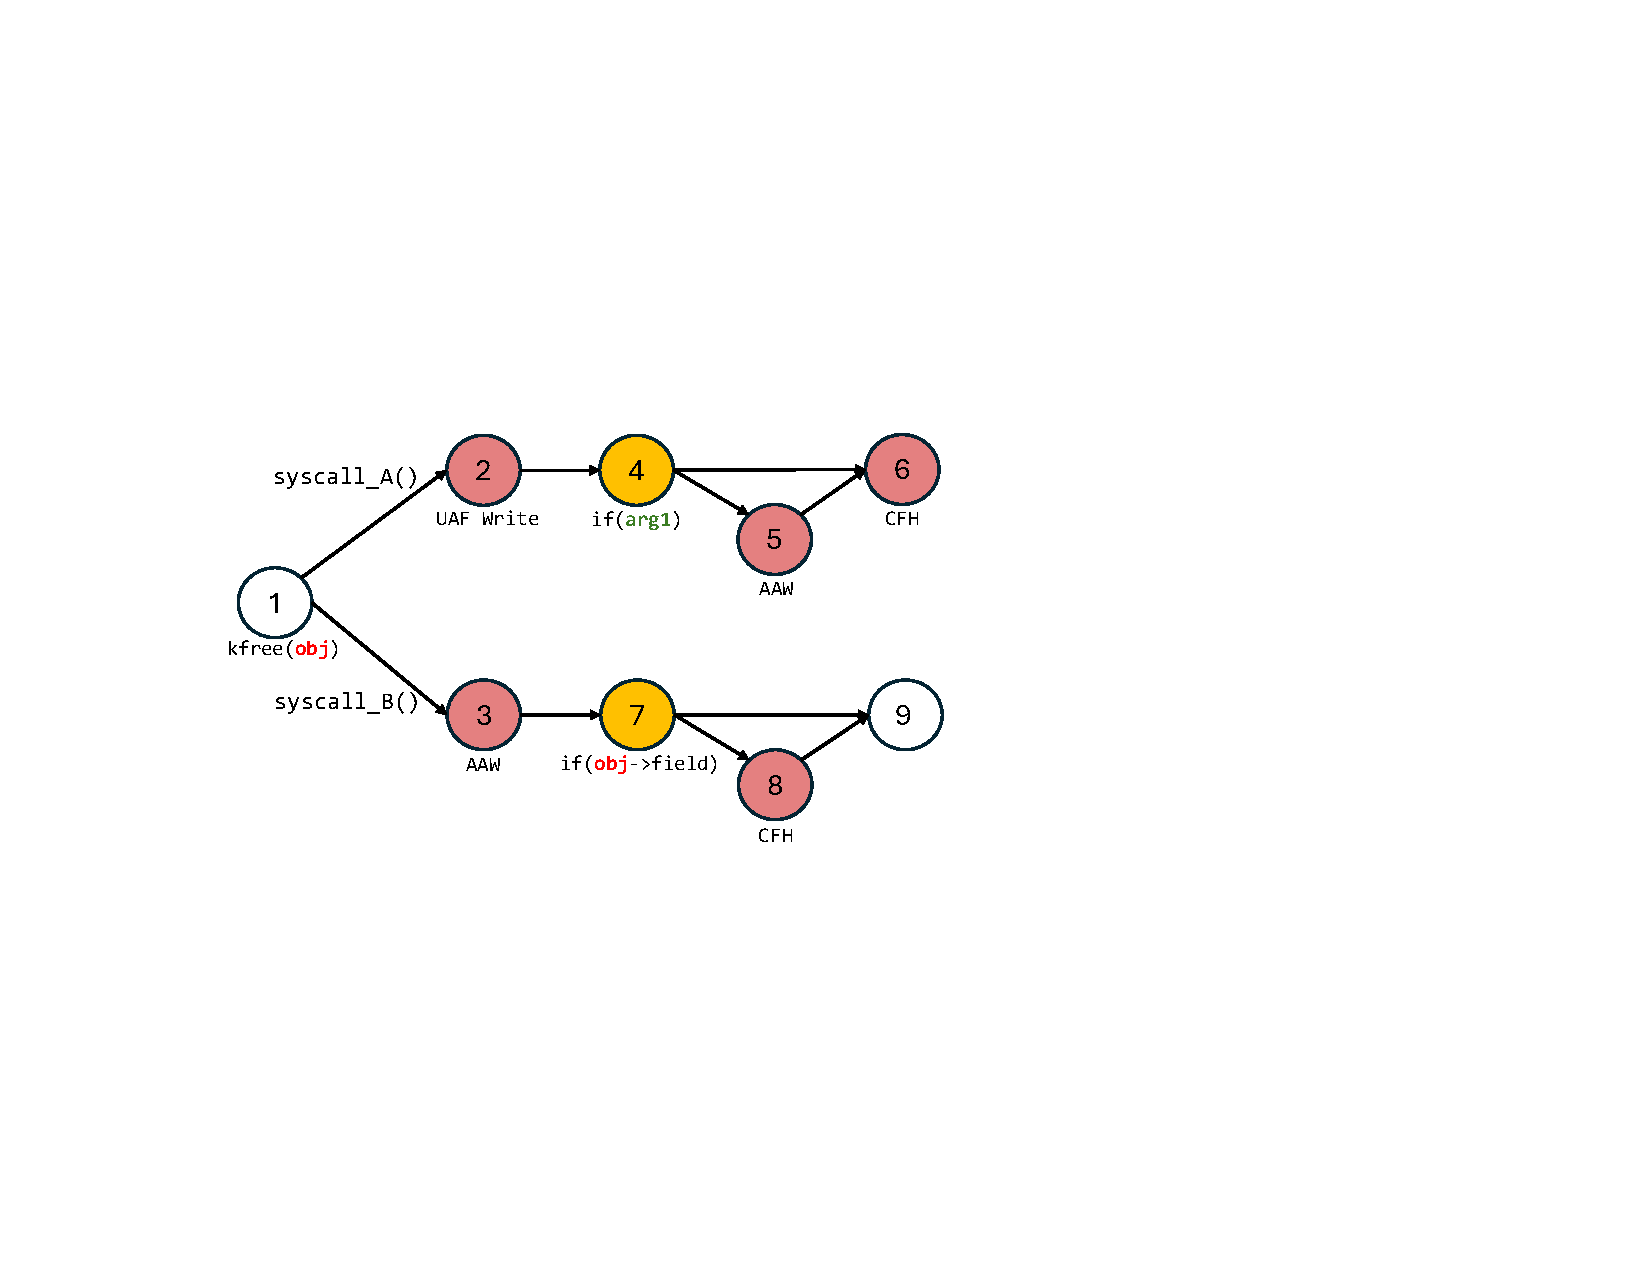
\includegraphics[width=\linewidth, trim=80 200 200 205, clip]{./figures/motivating.pdf}
  \vspace{-0.5cm}
  \caption{\label{fig:motivating}The motivating example kernel vulnerability}
\end{figure}
% \zhiyun{is this a control flow graph? need to explain}


The motivating example is a UAF bug simplified from a real kernel bug.
The corresponding kernel code can be found in Figure~\ref{fig:motivating_code}, and a control flow graph annotated with potential primitives is depicted in Figure~\ref{fig:motivating}. In this bug, \textcolor{red}{\texttt{obj}} is freed, illustrated at \circled{1} in Figure~\ref{fig:motivating}, but there are two potential syscall invocations (\texttt{syscall\_A()} and \texttt{syscall\_B()}) that can still access a dangling pointer, leading to a use-after-free bug.

% \zhiyun{The description of the example is incomplete. We need to explain there are multiple primitives associated with different syscalls. Within each syscall, there are also multiple primitives --- reachable via different paths. Then we can explain why there may be side effects, if we want to choose, say the CFH primitive for exploitation. In fact, I think we will need some pseudocode to illustrate this. I drafted the beginning of a new paragraph below.}

As we can see from the simplified syscall implementations in Figure~\ref{fig:motivating_code}, an attacker can invoke \texttt{syscall\_A()} to potentially trigger 3 primitives: UAF Write, Arbitrary Address Write (AAW) and Control Flow Hijacking (CFH). On the other hand, invoking \texttt{syscall\_B()} will potentially trigger 2 primitives: AAW and CFH.

To influence the behaviors of the vulnerability and steer the kernel into different execution paths, the attacker can choose the bug-triggering syscall (i.e., \texttt{syscall\_A()}, \texttt{syscall\_B()}, or modify syscall arguments such as \textcolor{DarkGreen}{\texttt{arg1}} to alter the vulnerability context. Furthermore, the attacker can leverage heap spray to manipulate the memory pointed to by the dangling \textcolor{red}{\texttt{obj}} pointer, thereby influencing the execution paths in \texttt{syscall\_B()}.

Suppose the attacker’s goal is to hijack kernel control flow using a CFH primitive. One option is to invoke \texttt{syscall\_A()} and spray attacker-controlled data to reclaim the freed memory. However, this path deterministically triggers UAF Write at \circled{2}, and may also trigger an AAW at \circled{5}. 
%Here, \emph{AAW side effect} denotes an undesirable effect in which a pointer corrupted by sprayed data is dereferenced (the attacker may not know a valid address to place in that pointer field).
Both can crash the kernel. UAF Write may corrupt critical fields of the reclaimed object, causing later failure when that object is used. AAW is more severe, because dereferencing a corrupted pointer (e.g., \texttt{obj->p1}) can immediately fault if it points to an invalid address.

% \zc{Only an intended AAW by the attacker is called AAW; "AAW" side effect should be called dereferencing invalid write pointer, as the attacker has no intention to specify the address}\juefei{Changed}
%In this scenario, AAW \circled{5} is considered a primitive, and CFH \circled{6} is considered a side effect, as the attacker only wants to use AAW to corrupt the global variable and he does not want to alter the kernel control flow.
% Along these potential execution paths, there are effects such as UAF Write, Arbitrary Address Write (AAW), Control Flow Hijack (CFH).

\subsection{Effects, Primitives, and Side Effects} \label{chap:eps}

We begin by defining key terms that set the foundation for the rest of the paper.

\textbf{Effects} refer to any unintended memory operations directly or indirectly caused by the vulnerability.

\textbf{Primitives} are a subset of effects, denoting the specific effects that attackers choose to carry out an exploit. In the motivating example, if the attacker selects the CFH effect, e.g., to conduct return-oriented programming, we consider the CFH effect a primitive. Meanwhile, 

\textbf{Side effects} are defined as the remaining effects that occur together with the primitive, but are not chosen for exploit construction.

We make three key observations about these definitions.

\noindent\textbf{1. Primitives Are Chosen}: Whether an effect is considered a primitive depends on the attacker's strategy. For example, although CFH is often seen as powerful (e.g., for ROP), if the attacker chooses to use UAF Write instead (to corrupt heap objects), the CFH would become a side effect, which can lead to crashes if we do not overwrite it with a legitimate kernel function address.

\noindent\textbf{2. Primitives are Mutually Exclusive}: 
Attackers typically use a single primitive per bug trigger, since different primitives require distinct memory layouts that are difficult to realize simultaneously. When multiple primitives are needed, attackers usually retrigger the bug in separate executions. Therefore, once one primitive is selected in a given execution, the remaining effects are treated as side effects.

\noindent\textbf{3. Some Side Effects Are More Lethal}: 
Not all side effects are equally harmful. Side effects involving pointer dereferences are especially dangerous because they can fail immediately when the corrupted pointer field is filled with an invalid value (e.g., 0x0 from zero-initialized spray objects). For example, CFH and AAW are typically riskier than UAF Write: if the reclaimed object is zero-initialized and a pointer field is dereferenced without validation, the kernel will crash.

%\zhiyun{need to define purified primitives or clean primitives. I personally prefer clean because purified assumes it requires work to be clean (but a primitive may naturally be clean and does not require purification).}

%\zhiyun{The definitions here are much clearer (and more reasonable) than the ones in the opening paragraph. We should improve the opening paragraph to match the actual definition.}

%As a result, in this paper, we \textbf{do not} determine primitives based on the behaviors of effects. Instead, we leave the freedom of choosing the exploit strategy to the exploit developer and treat all effects as potential primitives equally. Thus, for each of them, we try to find strategies to solve other effects for it. In addition, we prioritize solving side effects involving pointer dereferences.

In this paper, we \textbf{do not} determine primitives from behaviors of effects. Instead, we leave exploit-strategy selection to the developer and treat all effects as equally viable candidate primitives. For each candidate, we then seek mitigation strategies for the remaining effects (i.e., side effects). We further prioritize mitigating side effects that involve pointer dereferences.


% For each potential primitive provided by the vulnerability, we assume the attacker chooses it as the primitive for the exploit, then treat all other unintended memory operations as side effects to be minimized


% Whether an effect is useful is largely subjective, depending on the attacker's strategic preferences. In our motivating example, all three effects might be chosen as the primitive for exploit development. UAF Write can be used to corrupt critical fields of other heap objects, AAW can be used for corrupting global variables, and CFH can be used to conduct ROP. However, regardless of which effect is chosen as the primitive, others effects becomes useless and then become side effects due to their contrary to the chosen exploit strategy. 


% In the motivating example, both AAW and CFH are generally viewed as promising effects. An experienced attacker may either choose AAW as the primitive and tamper critical global variable or choose CFH as the primitive and conduct ROP to achieve privilege escalation. However, regardless of which primitive is chosen, others effects becomes side effects.

% And side effects caused by AAW and CFH are especially fatal since involved pointer dereference and the risk of kernel crash. From the attacker's perspective, side effect \textbf{avoidance} and \textbf{neutralization} are two generic approaches dealing them.


% Furthermore, SyzScope does not associate the primitive with execution trajectory after triggering it (i.e., \circled{5}$\rightarrow$\circled{6}, \circled{3}$\rightarrow$\circled{7}$\rightarrow$\circled{9}, \circled{3}$\rightarrow$\circled{7}$\rightarrow$\circled{8}$\rightarrow$\circled{9}), completely missing effects after behind each primitive. Consequently, SyzScope's primitive reports provide very limited help for attackers.

% its report often lacks enough practicality to guide the attacker to develop an exploit. First, for each primitive, SyzScope only reports its exist and the first path SyzScope found towards it. For instance, for the AAW primitive, it may only reports \circled{1}$\rightarrow$\circled{3} 

% First, for each primitive, SyzScope only reports the first path to reach it, without alternative paths to reach it, and does not reason for paths after it. For instance, for the AAW primitive, it only reports \circled{1}$\rightarrow$\circled{3} or \circled{1}$\rightarrow$\circled{2}$\rightarrow$\circled{4}$\rightarrow$\circled{5} (based on which one is firstly executed) not both of them. And SyzScope does not reason whether the path can safely reach the end of syscall without triggering additional side effects. 

% First, for each primitive, SyzScope only reports the first path it discovers reaching it, failing to analyze other alternative paths with fewer side effects in a holistic way. For instance, for the AAW primitive. It only reports \circled{1}$\rightarrow$\circled{3}

% Second, SyzScope implicitly assumes the attacker can forge arbitrary level of kernel pointers to exploit the vulnerability, overly simplify the modeling of side effects. However, in practice, the attacker has limited ability to forge the kernel pointers, and report that requires the attacker to forge such pointer become meaningless


% Introduce side effect here


% How SyzScope would do that and How GREBE would do that

% In fact, these represent everything the attacker can control in the scenario of exploit development. Therefore, an effective side effects mitigation strategy must be based on either (1) adjusting the syscall or (2) manipulating the sprayed memory.

% It is a UAF bug, where the object is freed at \circled{1}, but can be used later.

% in the implementation of the \texttt{AF\_PACKET} socket within the \texttt{net} subsystem. The affected object is the \texttt{sk\_buff}, which represents a packet in the Linux kernel.

% The vulnerability arises from the mishandling of packets received through the \texttt{AF\_PACKET} socket. This error causes the kernel to free an \texttt{sk\_buff} object while leaving it in the doubly linked list associated with the socket. Therefore, as shown in Figure~\ref{fig:motivating}, an attacker can trigger the vulnerability in different ways by using various syscalls to interact with the socket.
% % To influence the behavior of the vulnerability, the attacker can change the syscall they execute to achieve that. Meanwhile, the behavior of the vulnerability is also influenced by syscall arguments, such as \textcolor{DarkGreen}{\texttt{flags}} and \textcolor{DarkGreen}{\texttt{len}}. Additionally, an attacker can also leverage heap spray to manipulate the memory pointed by the dangling \textcolor{red}{\texttt{skb}} pointer, and thus influence the behavior of the vulnerability.

% To influence the behavior of the vulnerability, the attacker can choose a different syscall. Meanwhile, the behavior of the vulnerability is also influenced by syscall arguments, such as kernel variables \textcolor{DarkGreen}{\texttt{flags}} and \textcolor{DarkGreen}{\texttt{len}}, which are controled by the syscall argument. Additionally, an attacker can leverage heap spray to manipulate the memory pointed to by the dangling \textcolor{red}{\texttt{skb}} pointer, thereby influencing the behavior of the vulnerability. 

% In fact, these represent everything the attacker can control in the scenario of exploit development. Therefore, from the attacker's perspective, effective side effects mitigation strategies should focus on two primary approaches: (1) adjusting the syscall, and (2) manipulating the sprayed memory.





% 1. Side effect avoidance via Syscall Manipulation

% 2. Side effect avoidance via Sprayed Memory

% 3. Side effect neutralization.

\section{Overcoming Side Effects}
In this section, we illustrate avoidance and neutralization as two generic strategies for solving side effects under the motivating example. We further analyze the limitations of existing primitive discovery frameworks under side effects.

\subsection{Side Effect Avoidance} % via Syscall Adjusting 
% Make subsubsec about syscall/spray

% In the motivating example bug, The attacker can adjust the syscalls or their arguments to change the context of the vulnerability \cite{zou2022syzscope}. Thus, syscall adjusting can naturally influence the vulnerability behaviors and avoid side effects.

The most intuitive way to mitigate side effects is to identify \textit{alternative execution paths} that avoid triggering them while still triggering the desired primitive. However, since an attacker does not know ahead of time which primitive to pick for exploitation and which effects would become side effects, it is generally a good idea to explore as many alternative execution paths as possible. In particular, there are two kinds of attacker-controllable input in an exploit that can determine the execution path: (1) syscall sequence and arguments, and (2) memory contents introduced through heap spraying. Both can influence the execution path. We thus further categorize the side effect avoidance into the following two types:

\vspace{0.015in}
\noindent\textbf{Avoidance by Syscall Adjustments.}
Syscall adjustments can change the context in which a bug is triggered ~\cite{zou2022syzscope}. This context shift may invoke a different vulnerability-triggering function, resulting in substantial changes in vulnerability behavior. In other cases, the effect is subtler: syscall changes perturb only local variables yet still influence control-flow decisions far from the initial memory corruption site. Overall, these context-induced variations can aid side-effect avoidance by steering execution onto alternative paths.

% Thus, an attacker can carefully craft the vulnerability triggering syscall sequence to prevent the kernel from entering side effect triggering code, thus avoiding side effects.

Going back to the motivating example and Figure~\ref{fig:motivating}, if the attacker intends to leverage the CFH primitive to exploit the vulnerability, regardless of whether it is in \texttt{syscall\_A()} or \texttt{syscall\_B()}, there is a corresponding AAW effect can be a side effect and needs to be avoided.

To do so, the first observation is that \texttt{syscall\_A()} is better than \texttt{syscall\_B()}, since the AAW effect at \circled{3} is unavoidable when using \texttt{syscall\_B()}. In contrast, the AAW effect at \circled{5} can be avoided if the arguments of \texttt{syscall\_A()} are adjusted properly, i.e., by setting \textcolor{DarkGreen}{\texttt{arg1}} to zero, which can influence the \texttt{if} statement at \circled{4}, and thereby bypassing the AAW side effect at \circled{5}.

\vspace{0.015in}
\noindent\textbf{Avoidance by Memory Spraying.}
When a vulnerability is triggered, the kernel enters a ``weird machine'' state \cite{weirdmachine}. In this state, the code no longer follows its intended behavior. Instead, it accesses unintended memory regions, including areas belonging to attacker-sprayed kernel memory, which can also alter the control flow and potentially avoid side effects.
%So the attacker can leverage heap spraying and heap feng shui techniques to guide unintended memory accesses to the sprayed memory, redirecting the control flow to avoid side effects.

Suppose, in the motivating example, the attacker wants to develop an exploit by leveraging an AAW primitive, which means that the CFH becomes a side effect and should be avoided. Looking at \texttt{syscall\_A()} and \texttt{syscall\_B()}, we can see both have an AAW primitive. However, \texttt{syscall\_A()} is less preferred in this case because the CFH primitive cannot be avoided, unlike in \texttt{syscall\_B()}.


To avoid the CFH side effect in \texttt{syscall\_B()}, the attacker first creates a dangling \textcolor{red}{\texttt{obj}} pointer, then sprays memory so the bytes overlapping \textcolor{red}{\texttt{obj}}\texttt{->field} are \texttt{0x0}. When \texttt{syscall\_B()} is invoked, execution at \circled{7} follows \circled{9} instead of \circled{8}, thus avoiding CFH.


% the attacker invokes \texttt{syscall\_B()} and seeks to avoid CFH at \circled{8}. To prevent the kernel code from stepping into \circled{8}, the attacker expect \textcolor{red}{\texttt{obj}}\texttt{->field} be zero. Since \textcolor{red}{\texttt{obj}} is a dangling pointer, its value can be controlled by the attacker via heap spraying. Thus, with this knowledge, the attacker can carefully craft sprayed memory content and nullify \textcolor{red}{\texttt{obj}} to avoid the CFH side effect at \circled{8}


% the attacker can manipulate its content by memory spraying and nullify \textcolor{red}{\texttt{obj}}\texttt{->field} to make the kernel jump over \circled{8} and avoid side effects. 

\subsection{Side Effect Neutralization}
In addition to avoidance, side effects can also be addressed through neutralization, a strategy that allows side effects to occur while minimizing their consequences. In our setting, the primary objective is to prevent invalid memory accesses caused by invalid pointer dereferences that could lead to a kernel crash.


In the motivating example, suppose the attacker wants to exploit the CFH primitive. Instead of calling \texttt{syscall\_A()} to avoid the AAW side effect, the attacker can invoke \texttt{syscall\_B()} and neutralize the AAW at \circled{3}. 

To make AAW safe, the attacker must provide a valid writable kernel pointer at the dereference site. A standard approach is to spray objects with a pointer field at the exact dereferenced offset \cite{SETTLERS66:online,Onedaysh20:online}. By selecting the spray object layout, the attacker places a valid kernel address there, which becomes the write target and avoids an invalid dereference.

% In practice, attackers identify and verify suitable spray targets through manual analysis~\cite{SETTLERS66:online}.






% In our motivating example, if the attacker plans to exploit the CFH primitive, instead of using \texttt{syscall\_A()} to avoid the AAW effect, an alternative effective approach is invoking \texttt{syscall\_B()} but neutralize the AAW effect at \circled{3}. For such an AAW effect, the attacker needs to feed a valid kernel pointer to the code to ensure the AAW effect happen without crashing the kernel. The typical way of doing this is 
% when choosing the memory object to spray, the attacker chooses the one with suitable memory layout, where a valid writable pointer reside and will be used in the AAW under proper heap feng shui.In practice, attackers typically identify and verify such objects manually through extensive analysis \cite{SETTLERS66:online}.




% with \texttt{syscall\_B()} without crashing the kernel, they is to find a memory object with a pointer placed at the suitable memory offset,  



% \subsection{Sprayed Memory Manipulation}
% When a vulnerability is triggered, the kernel can enter a “weird machine” state \cite{weirdmachine}. Under such circumstances, code no longer behaves according to the kernel's original design, instead, it fetches memory that it shouldn't access and influenced by these memory. Thus, the attacker can spray memory objects and alter the vulnerability's behaviors to bypass side effects. In particular, by memory spraying, the attacker can apply two approaches two avoid or mitigate side effects:


% \noindent\textbf{1. Influencing Execution Path with Crafted Sprayed Memory.}


% \noindent\textbf{2. Neutralizing Side Effects with Suitable Memory Objects.}










% Despite  \texttt{recvfrom()} to trigger the vulnerability, the \texttt{\_\_skb\_unlink(skb)} still appears unless the attacker set \texttt{MSG\_PEEK} in the syscall argument to make \textcolor{DarkGreen}{\texttt{flags}} 

% To avoid \texttt{\_\_skb\_unlink(skb)}, the attacker needs only to use \texttt{recvfrom()}  to trigger the vulnerability, they also need to set the \textcolor{DarkGreen}{\texttt{flags}} parameter as \texttt{MSG\_PEEK} in the syscall argument. 

% Despite triggering the bug with \texttt{close()} may grant the attacker with control flow hijack capability by forging the \texttt{skb->destructor} function pointer. If the attacker plans to exploit the vulnerability with control flow integrity (CFI) enabled or simply can not find suitable return oriented programming (ROP) gadget, the attacker  


% Goal oriented
% \subsection{Exposing more effects}
% So many syscalls, we can't do symbolic execution on that, so still, we need do fuzzing to expose more effects. The more effects we discover, the higher chance that one of them being useful.

% \subsection{Path Exploration}
% Symbolic execution on fuzzed results. But we are doing it in a way that aims to avoid side effects.
% \subsection{Side Effects Avoidance}
% % Fuzz+SymExec
% %Fuzz: lowerbound effects? A+B+C effects vs A & B Only
% The most straightforward way to conquer side effects is to find an alternative feasible path that simply does not trigger side effects. To achieve this, an attacker can either adjust syscalls and their arguments to change the way the bug being triggered or manipulate sprayed memory to steer the weird machine after triggering the bug.

% \subsubsection{Branch Set Differentiated Fuzzing}

% To find different ways to trigger the bug, we need to explore the vast search space of syscalls and arguments. Fuzzing can mutate syscalls and arguments based on the original PoC, being demonstrated capable of discovering hidden primitives of the same bug.\cite{zou2022syzscope} \cite{lin2022grebe} \cite{tan2023syzdirect}. 

% However, existing fuzzing technique is not fine grained enough to serve the purpose of side effects avoidance. It wouldn't differentiate two variants of PoC if their first error behavior is the same, even if they'll behave drastically differently after that. As a result, different variants would be classified as the same PoC, stopping us from differentiating them and avoiding potential side effects.

% Take the example of the 380a bug \cite{380abug} in the motivating example, modifying the length of the syscall recv that triggers the use of the invalid SKB data seemingly wouldn't make a a difference, since the first error would be "\_\_skb\_try\_recv\_from\_queue+0x7c0/0x940". 

% \begin{lstlisting}[language=C]
% papstatic int packet_recvmsg(struct socket *sock, struct msghdr *msg, size_t len,
% 			  int flags)
% {
%     //Trigger the first error behavior
%     skb = skb_recv_datagram(sk, flags, flags & MSG_DONTWAIT, &err);
%     ...
%     packet_rcv_vnet(msg, skb, &len);
% }
% static int packet_rcv_vnet(struct msghdr *msg, const struct sk_buff *skb,
% 			   size_t *len)
% {
%     struct virtio_net_hdr vnet_hdr;
%     if (*len < sizeof(vnet_hdr))
%         return -EINVAL;
%     ...
%     //Pointer dereferences
%     virtio_net_hdr_from_skb(skb, &vnet_hdr, vio_le(), true, 0)
% }
% \end{lstlisting}

% However, different length argument passed into recv syscall would cause different execution flows, thus be able to avoid side effects in packet\_recvmsg since smaller offsets would be considered invalid, and not being used to copy data to the userspace,

% Thus, as a result, we proposed a novel technique named "Effect Aware Fuzzing". Instead of logging the first major effect of a same bug, our novel technique log the trace of KASAN report as a heuristic way to differentiate different bugs. 

% % To enlarge the search space, we should not stick to the original PoC, instead, we use kernel fuzzing technique to expose as more ways to trigger the bug as we can. However, different from traditional fuzzing technique 


% % Side effects avoiding is about manipulating data to not trigger side effects. This can be achieved by carefully selection of syscalls, arguments, and sprayed data. For a same vulnerability, there are multiple syscalls to trigger it, thus causing different effects. Thus, we may want to find the syscall and corresponding arguments with least side effects. However, static analysis based approaches introduce significant false positive which hinders precise analysis. Thus we chose fuzzing as our approach to discover potential ways to trigger the bug.

% % Exisisting works on fuzzing has serious problem of differentiate seeming similar seeds that trigger the same bug. 

% \subsection{Memory Layout Centered Side Effects Neutralizing}
% Matching with object.

\subsection{The Blind Spots of Existing Primitive Discovery Frameworks} 
\label{other_tool_problem}

A key blind spot of existing primitive discovery frameworks like GREBE and SyzScope is that they do not reason about side effects at all. These tools primarily focus on identifying as many observable effects as possible, treating them uniformly as usable primitives, i.e., all effects are considered potential primitives. However, not all such effects are equally exploitable, as we demonstrated in the motivating example. 
%some may interfere with others or introduce unintended consequences that render an exploit unworkable. 
Without analyzing the interactions between effects or accounting for side effects that can invalidate otherwise promising primitives, these frameworks risk presenting a misleading view of exploitability. In essence, they prioritize coverage and reporting over actionable guidance, leaving attackers to manually untangle the dependencies and constraints needed to handle side effects.


Let us consider an attacker who uses GREBE or SyzScope to find primitives and focuses on leveraging AAW primitives for exploitation. As a fuzzer-based framework, GREBE identifies that both \texttt{syscall\_A()} and \texttt{syscall\_B()} can trigger the bug, but leaves follow-up analysis to the attacker. SyzScope can successfully discover subsequent effects after the initial corruption, on either path \circled{1}→\circled{2}→\circled{4}→\circled{5} or \circled{1}→\circled{3}, depending on which is exercised first in its symbolic execution. However, three design-level limitations prevent them from analyzing side effects or offering practical guidance for exploit development.



\noindent\textbf{1. Low Sensitivity in Exploring Vulnerability Contexts:} Both frameworks mutate the original PoC to explore new contexts, detecting significant changes like a different triggering function in vulnerability contexts. This allows them to find that both \texttt{syscall\_A()} and \texttt{syscall\_B()} can trigger the bug. However, they lack sensitivity to subtle changes in \textcolor{DarkGreen}{\texttt{args}}, which affect the context at \circled{4} after the initial corruption at \circled{1}. This limits their ability to discover alternative paths by adjusting syscall arguments.

\noindent\textbf{2. Incomplete Execution Path Exploration:} Although SyzScope sees multiple effects on one path, its incompleteness lacks support for sprayed memory manipulation-based avoidance. First, SyzScope only tracks the first path it exercises for a given primitive, rendering it potentially overlooking alternative paths leading to the same primitive. In this example, if path \circled{1}→\circled{2}→\circled{4}→\circled{5} is exercised first, the better path \circled{1}→\circled{3} is ignored and discarded (note that \circled{3} and \circled{5} are both AAW effects). Second, SyzScope does not enforce execution through syscall completion and therefore can miss behaviors, e.g., \circled{3}→\circled{7}→\circled{9}, failing to help address post-primitive side effects.

\noindent\textbf{3. Overestimation of Pointer Forging:} SyzScope, based on symbolic execution, assumes the attacker can forge arbitrary levels of kernel pointers in sprayed memory. This means that if all pointer dereferences, e.g., \texttt{*(obj->ptr)} or \texttt{*(obj->f->ptr)}, are all reported as primitives. However, when multiple such primitives or effects are present in the same execution path, some of them are bound to become side effects. Consequently, primitives and their associated paths found by SyzScope may be impractical for real-world exploits, because they do not attempt to neutralize such side effects by spraying appropriate heap objects.






% of \circled{1}→\circled{2}→\circled{4}→\circled{5} and \circled{1}→\circled{2}→\circled{4}→\circled{6} caused by the.




% Existing primitive discovery frameworks exhibit limitations in generating practical guidance. Since GREBE only catches the first memory corruption effect in each syscall sequence, it can hardly discover more effects behind it (e.g., CFH in the motivating example), let alone analyzing them. 

% SyzScope models memory operations behind the first memory corruption to uncover more primitives. For each primitive, SyzScope identifies its presence and provides a single associated path. Take the AAW primitive as an example, SyzScope reports its existence and a single potential path (i.e., \circled{1}→\circled{2}→\circled{4}→\circled{5} or \circled{1}→\circled{3}). However, several design level issues hampers its practicality:

% \noindent\textbf{1. Lack}


% SyzScope models memory operations behind the first memory corruption to uncover more primitives, but still face limitations. For each primitive, SyzScope merely identifies its presence and provides a single associated path with no attempt at deeper analysis. Take the AAW primitive as an example, SyzScope reports only its existence and a single potential path (i.e., \circled{1}→\circled{2}→\circled{4}→\circled{5} or \circled{1}→\circled{3}). This design limits the practicality of SyzScope.


% However, it provides no guarantee that the reported path's side effects can be resolved in practice. This is because SyzScope implicitly assumes the attacker can forge arbitrary levels of pointer indirection in the sprayed memory, neutralizing side effects silently. But this assumption does not hold in the real world. Moreover, SyzScope fails to link each primitive to its subsequent execution trajectory (e.g., \circled{5}→\circled{6}, \circled{3}→\circled{7}→\circled{9}, etc.), thereby missing the downstream effects behind the primitive entirely. As a result, SyzScope’s primitive reports offer very limited value for exploit development.


\section{SyzPass Design}
To overcome these shortcomings, we design SyzPass, a framework that comprehensively discovers primitives in vulnerabilities while automatically measuring and solving side effects residing in these primitives, generating actionable analyses to facilitate kernel exploit development. In this section, we illustrate the design of SyzPass, showing how it achieves automatic side effects solving.


\subsection{Workflow}

\begin{figure*}[htbp]
  \centering
  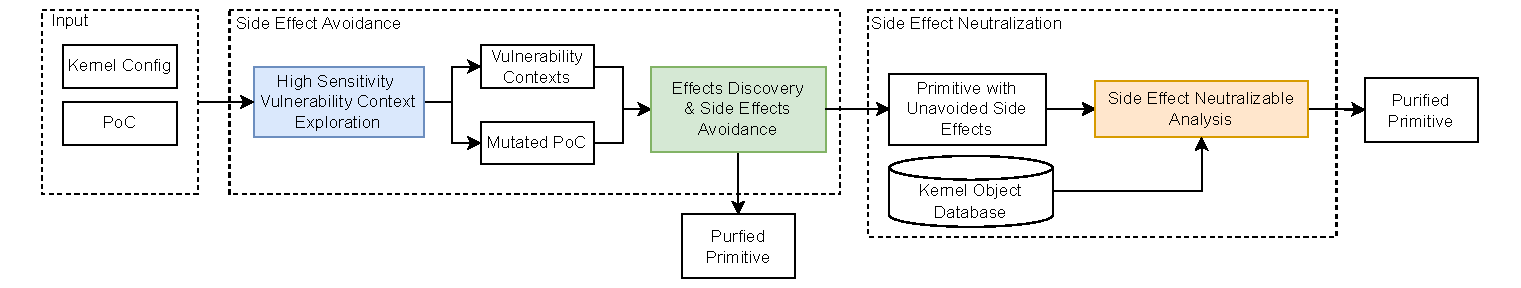
\includegraphics[width=0.99\linewidth]{figures/syzpass_pipeline.pdf}
  \caption{\label{fig:fuzz-graph}The workflow of SyzPass}
\end{figure*}

The workflow of SyzPass is shown in Figure~\ref{fig:fuzz-graph}. It takes as input the target kernel configuration and a PoC that triggers the vulnerability. The output is a set of primitives, each associated with a set of side-effect outcomes; a primitive may appear on a path that encounters zero or more side effects.
Furthermore, each side effect outcome is also tied to a corresponding strategy, including syscall sequences and sprayed data constraints for syscall avoidance, and kernel objects to neutralize residual side effects.

% primitives reside in the vulnerabilities and corresponding actionable side effects solving strategies consist of associated syscall sequence, data constraints for sprayed memory, and matched objects that can neutralize remaining side effects. 

Using the original PoC, SyzPass first explores vulnerability contexts to identify alternative syscall sequences that trigger the vulnerability, i.e., \emph{High Sensitivity Vulnerability Context Exploration}. It then explores execution paths after the initial corruption to search for alternative execution paths to avoid side effects, i.e., \emph{Primitive Discovery \& Side Effect Avoidance}.
For primitives where side effects are unavoidable, SyzPass examines memory layout requirements to neutralize them, i.e., \emph{Side Effect Neutralization Analysis}. Leveraging this analysis with a kernel heap object database that we collected, SyzPass matches suitable kernel objects to spray for neutralizing such unavoidable side effects.

% SyzPass first leverages high-sensitivity fuzzing to explore alternative vulnerability contexts the attacker can leverage. It then uses symbolic execution to analyze the possible execution paths that an attacker could manipulate the kernel to follow using memory spraying. Finally, it analyzes these paths and match associated data constraints with kernel memory objects to comprehensively apply  side effect avoidance and side effect neutralization to solve the side effects issue.


\subsection{High Sensitivity Vulnerability Context Exploration}
\label{sec:context_exploration}

The goal of the vulnerability context exploration component is to support syscall-adjustment-enabled avoidance. We leverage syscall fuzzing because it adjusts syscalls by design (e.g., sequence and argument values). On the other hand, it is significantly more difficult to fuzz attacker-sprayed memory, which is why we leave it to the next component.
%in exploring the vast search space of syscalls and arguments needed for context exploration. 

Prior work~\cite{lin2022grebe,zou2022syzscope,tan2023syzdirect,harbianqa,yome} employs fuzzing to explore targeted kernel areas. However, these approaches lack the sensitivity necessary to detect subtle changes in vulnerability contexts, as discussed in \S~\ref{other_tool_problem}. 

The primary reason is that most existing solutions are Syzkaller-based, retaining their original crash classification mechanism. However, the original mechanism determines that two crashes are the same if they share the identical initial corruption and bug-triggering function. While being effective for bug detection, this limits fuzzers' ability to identify subtle context changes behind the initial corruption, which can include additional effects, as illustrated in Figure~\ref{fig:motivating}. SyzScope makes a modification to this mechanism by identifying the first write-related corruption when the initial corruption is a read, and using it for crash classification. Unfortunately, it does not differentiate and record the various execution paths that may encounter different numbers or types of effects.
%\zhiyun{The description is not clear. Better use the motivating example to explain the subtle difference here.}

Therefore, we need to design an enhanced crash signature to enable more sensitive crash classification. Such an enhanced signature should distinguish seemingly identical crashes caused by different potential primitives and path constraints, while remaining efficient and robust. For such a mechanism, we propose three requirements: %\zhiyun{these requirements need to be explained with more details, e.g., examples. We can move pieces from later paragraphs here.}

\noindent\textbf{1. Sensitive:} It should be able to detect subtle context changes beyond the initial effect, which is critical for context exploration. For example, we should distinguish \circled{4}→\circled{5} from \circled{4}→\circled{6} in the motivating example (Figure~\ref{fig:motivating}).

\noindent\textbf{2. Noise Resilient:} One naive solution is to track post-initial-effect paths, which is the most sensitive.
However, this is susceptible to noise. Specifically, branches that are unrelated to the vulnerability may appear in the results. Additionally, branches associated with the vulnerability but unaffected by syscall arguments will also be included.
For example, the branches \circled{7}→\circled{8} and \circled{7}→\circled{9} would be differentiated under this approach, even though they are not influenced by the syscalls and should not factor into crash differentiation; instead, they should be differentiated by side effect avoidance by memory spraying (see \S\ref{sec:symbolic_execution}).

%While being sensitive, the mechanism must remain robust against noises, such as variables irrelevant to the vulnerability, memories influenced by heap spraying. This ensures the classification results remain stable.

\noindent\textbf{3. Efficient:} As classification is triggered on every crash and context exploration induces frequent failures, the classification mechanism must be lightweight. For example, if we were to track the influence of branches affected by syscalls (e.g., sequence and argument values), we would need to do so across the boundary of syscalls, due to dependencies among syscalls~\cite{dependency_measurement}. This can be prohibitively expensive, especially when conducted frequently. 
%tracing to identify whether a branch is influenced by syscall arguments or relevant to the vulnerability is highly unscalable, making it incompatible with our efficiency requirement. 
%\zhiyun{Efficiency of classification mechanism. Heavyweight due to cross-syscall tracing. That's why we have to resort to tracking symbolic memory instead of syscall arguments.}




%Due to our sensitivity requirement, our new mechanism must distinguish \circled{4}→\circled{5} from \circled{4}→\circled{6} in the motivating example. However, naively tracking all post-crash branches is susceptible to noise. Specifically, branches that are contextually related to the vulnerability may still appear in the results. Additionally, branches associated with the vulnerability but unaffected by syscall arguments are also included. For example, the branch at \circled{7} would be tracked under this approach, even though it is not influenced by the syscall sequence and should not factor into crash differentiation. Conversely, performing precise cross-syscall tracing to identify whether a branch is influenced by syscall arguments or relevant to the vulnerability is highly unscalable, making it incompatible with our efficiency requirement. 

To balance these requirements, we propose a lightweight branch set collection algorithm, as depicted in Algorithm~\ref{alg:effective-branchset}. Given a memory snapshot of the crashing kernel, the algorithm performs fast concolic execution to collect branches that are potentially influenced by syscall arguments.
%which serve as a complementary signature beyond the crash title.

% analyze every single crash, in order to differentiate crashes with new contexts. 
%It efficiently generates a set of context-relevant branches to facilitate crash differentiation.


\begin{algorithm}[htbp]
\caption{Efficient Branch Set Collection}
\label{alg:effective-branchset}
\begin{algorithmic}[1]
\Require Memory snapshot $S$
\Ensure  branch set $B$

\State $P \gets \emptyset$ \Comment{pending candidate branches}
\State $B \gets \emptyset$ \Comment{collected branch set}
\State $Bucket \gets \emptyset$ \Comment{map between IPDs and branches }
Symbolize(S)\Comment{symbolize UAF/OOB R memory }
% \State Symbolize heap-sprayed controllable memory in $S$

\While{execution continues}
    \State $rip \gets$ current instruction address

    \If{$rip \in \text{Bucket}$} \Comment{prune irrelevant branches}
        \State $P \gets P \setminus \text{Bucket}[rip]$
    \EndIf
    \If{$rip$ is a branch with unsymbolized condition}
        \State $(f, t) \gets$ jump from $rip$ to $target$
        \State $P \gets P \cup \{(f, t)\}$
        \State $ipd \gets \textsc{GetIPD}(f)$
        \State $\text{Bucket}[ipd] \gets \text{Bucket}[ipd] \cup \{(f, t)\}$
    \ElsIf{memory corruption operation is detected}
        \State $B \gets B \cup P$
        \State $P \gets \emptyset$
    \EndIf
\EndWhile

\State \Return $B$
\end{algorithmic}
\end{algorithm}

%Our key insight is that attacker influence on kernel execution primarily stems from two sources: memory spraying and bug-triggering syscall sequences. To avoid tracking the influence from syscalls, which is expensive due to the aforementioned cross-syscall challenge, we flip the problem by identifying branches \textit{affected} by memory spraying and avoiding using them to differentiate different crashes. 
Our key insight is that attackers mainly influence kernel execution through two channels: heap spraying and bug-triggering syscalls (including arguments). Because tracking syscall influence is expensive under cross-syscall interactions, we reverse the analysis: we detect spray-influenced branches and exclude them when distinguishing crash behaviors. This cuts overhead enough to run on every fuzzer-triggered crash.

Given that attackers mainly influence the execution (i.e., control flow) through two channels: syscalls and memory spraying, and the fact that tracking syscall influence is expensive (due to aforementioned cross-syscall interactions), our idea is to reverse the analysis.
Specifically, instead of identifying which branches are influenced by syscall arguments, we can identify spray-influenced branches and exclude them when distinguishing crash behaviors. This significantly reduces the analysis overhead, allowing this to be performed on every crash triggered by the fuzzer. 

To this end, we employ concolic execution by symbolizing UAF or OOB read memory. We detail the procedure in Algorithm~\ref{alg:effective-branchset}. As concolic execution progresses until the end of the syscall, we examine branches and their path constraints (if any) to extract the branch set.
If a path condition is not symbolized, i.e., not influenced by heap spraying memory (so that thus potentially influenced by bug-triggering syscall arguments), we add the corresponding branch into pending candidate branches \textit{P}, indicating that they are candidate branches for collection.

% The reason why these candidate branches are not directly merged into the final branch set \textit{B} is that we need an extra filter to exclude branches irrelevant to memory effects within this vulnerability.  
To exclude noise, we add candidate branches to the final set only when they are relevant to subsequent memory effects. We use the following heuristic: a branch is relevant iff at least one effect is control-dependent on it. Specifically, we apply \textit{immediate post-dominator} (IPD) analysis. The IPD of a branch is the first basic block guaranteed to execute regardless of branch direction; blocks after the IPD are not control-dependent on that branch. Therefore, if an effect occurs between the branch instruction and its IPD (i.e., it happens conditionally), we include it in the final branch set \textit{B}; otherwise, we treat it as noise and discard it.

% that are irrelevant to primitives beyond the initial crash\zhiyun{This sentence is difficult to parse. What is ``irrelevant to primitives'' and why ``beyond the initial crash''? I feel that we haven't given enough intuition about what we are trying to achieve here}. Thus, we apply \textit{immediate post-dominator} (IPD) analysis. The IPD of a branch is the first basic block that is guaranteed to execute after the branch, regardless of the direction taken. Thus, if memory corruption operations happen between a branch and IPD, the branch is considered to be potentially influential to it, and is merged to the final branch set \textit{B}; otherwise, the branch is treated as noise and ignored.

% This algorithm is efficient, as it yields results through concolic execution, and the computation of IPD is nearly linear.


% concolic execution by \textbf{symbolizing memory regions controllable via heap spraying}. During execution, branches with concrete (non-symbolic) conditions are considered unaffected by spraying, and are thus attributed to the syscall influence.


% While filtering out branches influenced by heap spraying helps reduce noise, it is not enough: many branches affected by syscall behavior may still be unrelated to the actual memory corruption. To more precisely isolate the control-flow decisions that are semantically relevant to the vulnerability, we apply \textit{immediate post-dominator} (IPD) analysis. The IPD of a branch is the first basic block that is guaranteed to execute after the branch, regardless of the direction taken.
% Our intuition is as follows: if execution reaches the IPD and no effects are triggered, then we say the branches taken did not contribute to the bug.



%While filtering out heap-spray-influenced branches already reduces noise, this alone is insufficient. Many syscall-influenced branches may still not contribute to the actual memory corruption. To further isolate only the branches that are semantically relevant to the vulnerability, we apply \textit{immediate post-dominator} (IPD) analysis. An IPD of a branch is the first instruction that always executes after the branch, regardless of which path is taken. Intuitively, if execution reaches the IPD without triggering memory corruption (e.g., UAF write), we conservatively discard the corresponding branch, since it does not influence whether the bug manifests. This enables precise pruning of irrelevant branches without relying on heavyweight dependency tracking.

With this new signature and fuzzing through mutation on the original PoC, we can effectively discover alternative syscall sequences for bug triggering, exploring vulnerability contexts in a highly sensitive manner, and setting foundations for subsequent analysis. 

\subsection{Effect Discovery and Side Effect Avoidance}
\label{sec:symbolic_execution}

\begin{figure}[htbp]
  \centering
  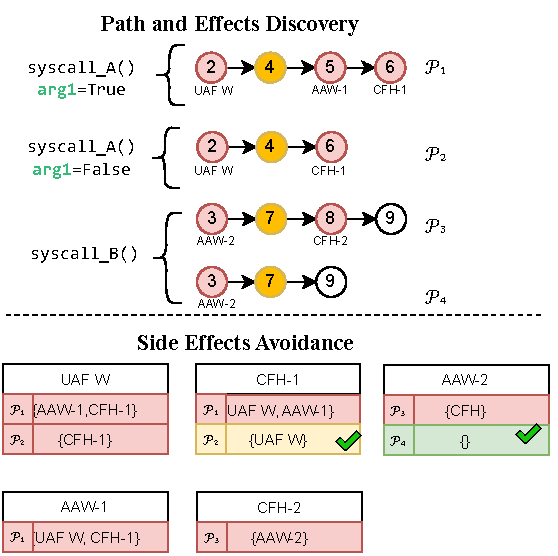
\includegraphics[width=\linewidth,trim=0 0 0 5, clip]{figures/symexec.pdf}
  \caption{\label{fig:symexec}Effects Discovery and Side Effect Avoidance}
\end{figure}

While the previous component explores various execution paths influenced by one source of attacker-controlled input, i.e., syscalls, this component focuses on paths affected by the other major input source: the attacker's sprayed memory.
In particular, this component employs symbolic execution by modeling the attacker's control over heap memory symbolically and analyzing potential memory effects and paths behind the initial corruption. 

Through symbolic execution, we perform fine-grained memory operation analysis to identify memory effects.
For example, if a \texttt{call} instruction targets a register containing symbolic data, we classify it as a control-flow hijack (CFH) effect.
Moreover, it also enables the exploration of alternative execution paths corresponding to each identified memory effect. Consequently, we can enumerate potential paths for each memory effect and perform side effect avoidance.

% This is crucial because additional effects may be discovered after the initial memory error, which has both positive and negative implications. On the one hand, more effects provide greater flexibility for primitive selection. On the other hand, observing multiple effects along a single execution path raises concerns about side effects. Knowing the complete set of effects associated with each path helps with side effect avoidance.

% Furthermore, along each symbolic execution path, we perform precise memory operation analysis leveraging the symbolic executor to identify potential effects. For example, if a \texttt{call} instruction targets a register containing symbolic data, we consider this a control-flow hijack (CFH) effect.

We illustrate this process through the motivating example in Figure~\ref{fig:symexec}. The upper part illustrates the paths and memory effects achievable through symbolic execution. The lower part summarizes, for each path, the set of associated effects. The red cells mark unresolved lethal side effects; yellow cells mark unresolved non-lethal side effects; green cells indicate no additional side effects on the path.


The symbolic execution starts with three vulnerability contexts (two \texttt{syscall\_A} related and one \texttt{syscall\_B} related) generated using the approach described in \S\ref{sec:context_exploration}. Notably, for \texttt{syscall\_B}, two paths $\mathcal{P}_3$ and $\mathcal{P}_4$ are discovered through symbolic execution.


% We assume the previous part context exploration component is finished with three PoCs generated (two \texttt{syscall\_A} related and one \texttt{syscall\_B} related). The advantage of using symbolic execution, for the PoC with \texttt{syscall\_B}, is that we can find both paths of  $\mathcal{P}_3$ and $\mathcal{P}_4$, not just one of them. This provides us more paths available and potentially more strategies for avoiding side effects.

% different potential paths of the motivating example vulnerability's different paths, as depicted in Figure~\ref{fig:symexec}. We start from 3 PoCs generated by the context exploration component. Suppose without heap spraying, their execution trajectory corresponds to $\mathcal{P}_1$ to $\mathcal{P}_3$. Using symbolic execution by symbolizing the attacker-sprayed memory, we find that it is possible to avoid the CFH effect, leading to $\mathcal{P}_4$.
%Finally, it is important that we record a set of execution paths (i.e., $\mathcal{P}_1$ to  $\mathcal{P}_4$) and the primitives associated with them.

% The second step is performing side effects avoidance. For analyze each potential primitive's associated paths, identifying those with minimal side effects to achieve side effects avoidance. For instance, for the AAW primitive, there are three paths $\mathcal{P}_1$,$\mathcal{P}_2$,$\mathcal{P}_3$ associated to it.  Since both $\mathcal{P}_1$,$\mathcal{P}_2$ contain pointer dereference related side effects, they then regarded fail to avoid side effects. Meanwhile $\mathcal{P}_3$ doesn't contain any side effects, so $\mathcal{P}_3$ is picked as the suitable path for the AAW primitive.

With these paths and associated effects mapped out, we can start triaging them and deciding on what effect(s) to choose as primitives. Ideally, for each potential primitive, we should pick a path with minimal side effects, as depicted in the lower half of Figure~\ref{fig:symexec}. In this example, if an attacker hopes to pick an AAW primitive, there are two options: AAW-1 from \texttt{syscall\_A()} and AAW-2 from \texttt{syscall\_B()}. The former has only one associated path: $\mathcal{P}_1$, and there are unfortunately two side effects, including a CFH. The latter has two associated paths $\mathcal{P}_3$ and $\mathcal{P}_4$, and $\mathcal{P}_4$ is completely free of side effects. Thus, $\mathcal{P}_4$ is the preferred choice for further exploit construction.

Similarly, if the attacker aims to select a CFH primitive, both syscalls offer viable options. However, CFH-1 associated with $\mathcal{P}_2$ (under \texttt{syscall\_A()}) would be the preferred choice, as its only associated side effect is a UAF write, which may not result in a crash and is therefore less likely to interfere with the exploit.
%In contrast, $\mathcal{P}_3$ contains no side effects and is therefore selected as the preferred path for this primitive. Thus, during the exploit development, the attacker can pick the $\mathcal{P}_3$ path to exploit the bug through the AAW primitive.


% To accurately model kernel behavior in weird machine states (i.e., after initial memory corruption happen), we leverage symbolic execution. With symbolized heap memory, we reason about how heap manipulations steer execution along different paths, and we perform precise memory operation analysis along these paths to identify potential primitives. Finally, with paths explored and primitives discovered, we analyze each potential primitive's associated paths, identifying those with minimal side effects to achieve side effects avoidance. We detail our key designs as follows.
Below, we describe the design of this component in more detail:

\noindent\textbf{1. Path Exploration:} For each vulnerability context associated with a PoC, we rerun the PoC to trigger the crash and take a kernel memory snapshot at the point of initial memory corruption. Using this snapshot, we symbolize the controllable heap-sprayed memory and initiate symbolic execution to explore subsequent execution paths. 

Unlike prior work, our analysis requires symbolic execution to reach the end of the bug-triggering syscall or interrupt handler. This is because we need to confirm the absence of side effects both \textit{before} triggering the primitive and \textit{after}. Thus, a complete execution path is required to expose all side effects associated with each primitive.

However, it can be expensive to explore every path till the end. To mitigate the scalability challenge, we design a pruning strategy based on how promising a path is, i.e., side-effect-free. In particular, we terminate symbolic states early when a memory access involves more than two levels of dereferences over symbolic pointers, e.g., \texttt{*(p->f->dp)} where p is a symbolic pointer. Deep pointer chains are unlikely to be satisfied by heap spraying in real-world attacks, making the corresponding paths ineffective (or at leat undesirable) for side-effect-free exploitation. %Therefore, such states can be safely pruned without compromising our analysis goals.

% In support of this strategy, we modify existing work's \cite{zou2022syzscope} memory model and customize for dereference depth tracking on symbolic pointers. detailed in Algorithm~\ref{alg:deref-depth}. During initialization, symbolic variables mapped to heap-sprayed memory are initialized with depth zero and marked.

In support of this strategy, we modify the existing work's \cite{zou2022syzscope} memory model and customize it for dereference depth tracking on symbolic pointers, detailed in Algorithm~\ref{alg:deref-depth}. Each symbolic variable from the heap-sprayed region is initialized with depth 0. When memory is accessed through a symbolic, unconstrained address, we assign a new symbolic variable to represent the pointer to the address, setting its depth to one plus the maximum depth among variables in the address expression. We then constrain this new variable to a dedicated dummy region to prevent repeated expansion.


% During initialization, symbolic variables mapped to heap-sprayed memory are initialized with depth zero. When a symbolic address points to previously unmarked memory, we create a new symbolic variable for that region and assign it a depth equal to the maximum depth among all symbolic variables in the address expression, plus one. This process is detailed in Algorithm~\ref{alg:deref-depth}.

\begin{algorithm}[htbp]
\caption{Dereference Depth Tracking}
\label{alg:deref-depth}
\begin{algorithmic}[1]
\Require Snapshot $S$, symbolic region $R$
\Ensure Depth map $D$ for symbolic variables

\State Initialize depth map $D$ bound to state
\ForAll{$a \in R$}
    \State $v \gets \textsc{SymbolicVar}(a)$,\quad $D[v] \gets 0$
\EndFor

\While{execution continues}
    \If{accessed address $e$ is symbolic and unconstrained}
        \State $v \gets \textsc{SymbolicVar}(e)$
        \State $D[v] \gets \max\{ D[u] \mid u \in \textsc{Vars}(e) \} + 1$
        \State Constrain $v$ to dummy region
    \EndIf
\EndWhile
\end{algorithmic}
\end{algorithm}



% \begin{algorithm}[H]
% \caption{Pointer Dereference Depth Tracking}
% \label{alg:deref-depth}
% \begin{algorithmic}[1]
% \Require Symbolic state $s$, heap spray region $H$
% \Ensure Per-State Mapping $D$ from symbolic variables to depth

% \State $D \gets \emptyset$
% \ForAll{$a \in H$}
%     \State $D[\textsc{Sym}(a)] \gets 0$
% \EndFor

% \While{symbolic execution continues}
%     \If{access $e$ is symbolic and $e \rightarrow m$ is unmarked}
%         \State $v \gets \textsc{Sym}(m)$
%         \State $D[v] \gets \max\{ D[u] \mid u \in \textsc{Vars}(e) \} + 1$
%         \State Mark $m$
%     \EndIf
% \EndWhile
% \end{algorithmic}
% \end{algorithm}




\noindent\textbf{2. Primitive Discovery:} During symbolic execution, we inspect each memory operation to identify exploit primitives, following the definitions in prior work~\cite{zou2022syzscope}.
For every memory write, we classify primitives based on the target address and value: writes to symbolic addresses are categorized as Arbitrary Address Write (AAW) or Constrained Address Write (CAW); writes targeting heap-sprayed memory are denoted as OOB/UAF Write (OUW); writes with symbolic values are classified as Arbitrary Value Write (AVW) or Constrained Value Write (CVW). The arbitrariness of addresses and values is determined via SMT solving over the collected symbolic constraints.
In addition, we monitor function call targets and arguments to detect Invalid Free (IF) and Control Flow Hijack (CFH).
We exclude memory read operations from primitive collection, as they do not directly enable privilege escalation, though their access patterns and pointer dereferences are still tracked as side effects. 
%\zhiyun{I thought we consider only pointer dereferences as side effects?}

\noindent\textbf{3. Side Effect Avoidance:} With the collected paths and primitives, we devise strategies to avoid side effects by selecting, for each primitive, the execution path with minimal side effects, ideally no side effects.

A prerequisite for this comparison is to identify all execution paths corresponding to the same primitive. To achieve this, we establish a mechanism to associate instances of the same primitive across different paths by labeling them based on their type and the instruction address at which they occur. This is simple yet effective, and it supports comparing primitives across different vulnerability contexts.
%ensuring that semantically equivalent primitives are treated uniformly during analysis.

Once all paths associated with a given primitive are identified, we compute a side effect set for each path. Since we define side effects as all observable effects excluding a selected primitive itself, we construct each side effect set by subtracting the primitive
%and its corresponding pointer dereference constraints\zhiyun{what is the constraints here? did we introduce it before?} 
from the path's overall effect set. These side effect sets serve as the basis for comparison and selection, e.g., we can rank primitives based on the minimum number of associated side effects.

As discussed in \S~\ref{chap:eps}, pointer dereferences related side effects are particularly critical, as they lead to kernel crashes if mishandled. Thus, such side effects must be avoided or neutralized. Otherwise, a primitive associated with such side effects is considered unusable. In the next section, we discuss solutions to neutralize such side effects, if they cannot be avoided, e.g., all paths associated with a primitive incur such side effects.
%first de-prioritize any path whose side effect set includes such high-risk operations.

%We then analyze the generated sets to identify paths and rank order them according to the number of side effects, i.e., zero being the best. 
%As discussed in Section~\ref{chap:eps}, pointer dereferences related side effects are particularly critical, as they lead to kernel crashes if mishandled. Thus, we first de-prioritize any path whose side effect set includes such high-risk operations.
%\zhiyun{again, we need to be clear whether we consider only pointer dereferences as side effects.} 
%Among the remaining candidates, we select the path with the fewest residual side effects as the preferred execution strategy. 

%Through this process, we systematically leverage the explored vulnerability contexts and post-corruption execution paths to discover primitives and avoid side effects. In some cases, however, we may still want to consider primitives associated with non-ideal paths, i.e., those that exhibit pointer dereference-related side effects and are inherently unavoidable. For example, it is possible that all paths have the same kind of side effect for a particular primitive. To address these cases, we leverage side-effect neutralization technique, which we detail next.

\subsection{Side Effects Neutralization Analysis}
The key idea of side effect neutralization is to pair paths with unavoidable pointer dereference-related side effects with sprayable kernel objects. 
Our design is to convert the side effects associated with a path into a \emph{required} memory layout, and each candidate object into an \emph{object} memory layout. We then simply compare the two and determine whether it is a match. If so, we say the side effect can be neutralized by spraying the corresponding object.
%By leveraging the memory layout of these objects, side effects can be neutralized during execution. We convert each path's data constraints\zhiyun{what kind of constraints?} and pointer-dereference relationships and kernel objects into a unified memory layout representation for effective comparison. 
We detail our design below, starting with a unified memory layout representation to support the matching:

\noindent\textbf{1. Memory Layout Representation Design:} We design our memory layout representation as a nested structure, depicted in Figure~\ref{fig:memlayout}.

\begin{figure}[htbp]
  \centering
  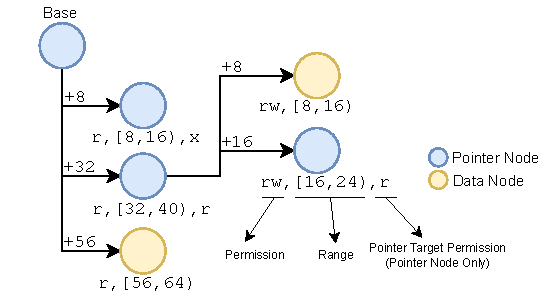
\includegraphics[width=\linewidth,trim=0 0 0 0, clip]{figures/memlayout.pdf}
  \caption{\label{fig:memlayout}Unified Memory Layout Representation}
\end{figure}

%\zhiyun{add a simple code example like if (valmem[56] $>$ 10) and explain how this is turned into a data node.}


In this representation, the memory layout is modeled as a tree, where each node represents a memory region (e.g., a field of an object). Each node is annotated with a byte range \([lo, hi)\), indicating the region's offset within the object, and an access permission field denoting the required memory access permissions.

Nodes are divided into two types. \textit{Pointer nodes} (blue) may point to another memory region in the layout and are annotated with an additional field: the target permission, which specifies the required permission of the pointee. This field allows us to simplify the tree by omitting the actual child nodes of the pointer when appropriate. Pointer nodes can have children, enabling the tree to recursively encode nested pointer relationships. The root node always represents a pointer to the kernel object (e.g., freed or accessed out-of-bounds) or the sprayed heap memory. Using the example in Figure~\ref{fig:memlayout}, we see the object associated with the root node has two pointer fields at two different offsets, i.e., 8 and 32, respectively. Furthermore, the object the second pointer points to has a pointer as well at offset 16.

\textit{Data nodes} (yellow) represent plain memory regions and are always leaf nodes in the tree. For these nodes, the byte range has special meanings. From the required memory layout side, the range indicates the memory whose values have to be specific. This is because of path constraints collected during symbolic execution. For example, there can be a conditional statement, such as \texttt{if(vulmem[56:64] > 10)}, whose true branch is taken in a path (e.g., to reach a particular effect). This results in the creation of a data node occupying the memory range [56, 64) within the required layout, as illustrated in Figure~\ref{fig:memlayout}. From the object memory layout side, a similar data node can be created if we know the corresponding memory value is controllable by an attacker, e.g., a buffer that can be initialized via syscall arguments.

Under this design, we can model nested pointer dereference chains to achieve object pairing. Furthermore, the concept of data nodes enables us to satisfy data requirements matching as well. These are the two most critical matching criteria we have observed in practice.

Lastly, there is a size annotation of the tree (not shown in the figure), indicating the total size of the kernel object or the sprayed heap memory. This size can provide a hint about which SLUB cache the vulnerable object belongs to, which will be helpful for object pairing. 


%pairing memory regions requiring constraints with controllable parts of spraying objects, increasing the practicality of matching.

\noindent\textbf{2. Required Memory Layout Construction:} For each path containing one or more side effects (pointer dereference), we construct a required memory layout using a three-phase process depicted in Figure~\ref{fig:memlayout_path}.


\begin{figure*}[htbp]
  \centering
  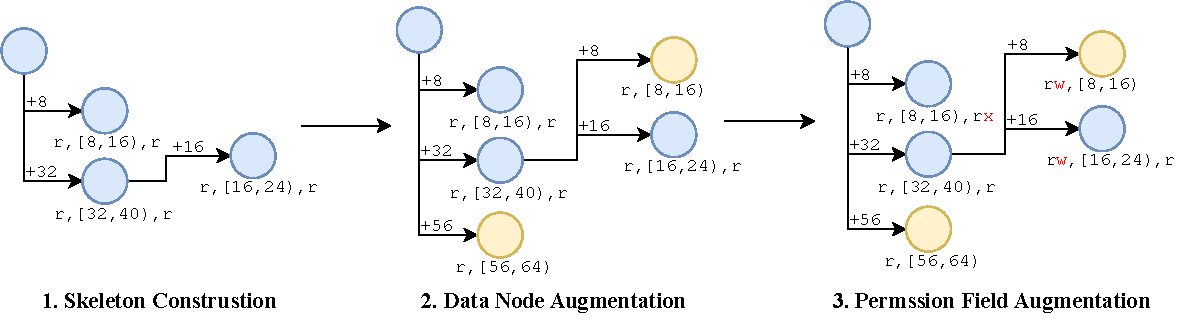
\includegraphics[width=0.9\linewidth,trim=0 5 0 0, clip]{figures/path_layout_creation.pdf}
  \caption{\label{fig:memlayout_path}Memory Layout Construction for Execution Path}
\end{figure*}

We initialize the tree and annotate the vulnerable object size information extracted from the KASAN report. Using this layout tree, we start the first phase, skeleton construction, where we capture pointer dereference relationships and initialize the tree. We iterate over symbolic pointer creations to identify newly introduced symbolic pointers and their corresponding base pointers, whose values are used to compute the new addresses. The relative offset is obtained by evaluating the difference between the new pointer's address and the base pointer's value using the symbolic solver. With the offset, we can generate the range needed for the attribute of the node. 
%For heap-spraying controllable memory, we designate its base pointer as the root node of the layout tree and calculate the offset by subtracting its address from the boundary of the sprayed memory region. Each such pair is added to the layout tree as a pointer edge, with default permissions initialized to read. 

Next, we traverse the remaining data constraints to augment the layout with data nodes. For each constraint, we identify the pointer used to access the memory region, compute the offset from the pointer’s base value to the target address using the solver, and determine the accessed byte range based on the data size of the related symbolic variables. A corresponding data node is then added as a child of the pointer node in the layout tree.

Finally, we parse the memory effects list of the path, augment write and execute permission among the layout tree based on the effect type and recorded constraint values.

Note that, as an optimization, we can first construct a tree for all effects on a path. Then, depending on the primitive picked, its corresponding nodes can be removed. 
%To further modify the layout for the need of the primitive, we trim the tree to exclude the current primitive from it, leaving it not used for comparison and neutralization. For a typical pointer dereference-related primitive, we achieve this by deleting the corresponding node and their children among the tree. 




\noindent\textbf{3. Memory Layout Reconstruction for Objects:} We collect objects among existing object databases from prior work to achieve memory layout reconstruction \cite{chen2019slake,chen2020systematic,wang2023alphaexp}, and assume them as sprayable and exploitable. To pair these objects with a required memory 
layout, we develop a simple algorithm to construct the object memory layout information through statically analyzing the kernel. In short, we parse the layout information of each structure to pinpoint pointers, then we iteratively generate the layout for pointers to model the pointer-dereference relationship. 

Following prior analysis of attacker-controllable fields in kernel objects~\cite{chen2020systematic}, we enrich object layouts with data nodes to represent memory regions that are considered user-controllable. In this context, a data node denotes an object field whose content can be influenced by the attacker. 


\noindent\textbf{4. Object Pairing for Side Effects Neutralization:} Our object pairing process consists of two phases. The first mode performs strict matching, requiring both data nodes and pointer dereference chains to match for precise analysis. However, if data node matching fails, it is also reasonable to consider a relaxed mode that only considers the pointer dereference structure for approximate matching. This is also useful since the exploit developer can perform manual analysis to understand whether the data constraints can be satisfied without requiring attacker-controllable memory specifically. For instance, if the data constraint requires some part of the vulnerable memory to be greater than or equal to zero, it is likely satisfiable by many objects naturally. We leave more precise data constraint solving as future work.

In both modes, we trim the primitive from associated path layouts to prevent the matching to neutralize the primitive, ensuring its exploitability. Then we match path layouts with object layouts one by one. Specifically, we check whether the required layout can align with the object layout without violating structural or permission constraints. For each pointer node in the path layout, we search for a matching node in the object layout that (i) covers an equal or greater byte range, (ii) provides equal or greater permission.
%\zhiyun{I don't understand what we mean by ``preserving the relationship''}
If a matching node is found, we recursively compare its children, following the pointer chain. In strict mode, we also require data nodes in the path to be matched precisely by data nodes in the object. 
%In relaxed mode, data nodes are ignored, allowing broader but potentially less precise matches.

A successful match means all pointer dereference side effects in the symbolic execution path can be safely neutralized using the object's memory layout. This lets the exploit generation continue without causing access violations or corrupting other kernel data. In such cases, we consider the neutralization successful and include the corresponding primitive, path, and matched object in our final output.


\section{Implementation}
\noindent\textbf{1. Vulnerability Context Exploration.}  
We extend Syzkaller and develop a concolic execution server based on Angr~\cite{shoshitaishvili2016sok} to support vulnerability context exploration. Syzkaller communicates with the concolic server via HTTP requests during fuzzing.

Upon VM boot, the customized syzkaller issues a request to the concolic server, providing the VM’s GDB port. The server sets a breakpoint at the kernel's KASAN report function to capture memory corruptions. When a corruption is detected and the breakpoint is triggered, the server symbolizes the KASAN-reported memory region and constrains the symbolic state using the original concrete data to initiate concolic execution and generate branch sets. Simultaneously, after observing the KASAN output, syzkaller queries the server to retrieve the generated branch set.

To ensure that fuzzing remains within the vulnerability context, we customize syzkaller’s mutation strategy by restricting mutations to the original PoC and its reproduced variants. The allowed syscall set is also confined based on the original PoC. This mutation strategy is consistent with prior efforts~\cite{zou2022syzscope}.
%and integrates naturally into our overall pipeline.

To conduct immediate post-dominator computation, we implement our own intra-procedural control-flow-graph (CFG) construction algorithm to avoid using Angr's heavyweight whole-program CFG generation mechanism. Specifically, we transform the graph and leverage \texttt{networkx}\cite{hagberg2008exploring} to compute immediate post dominators.

We further improve fuzzing efficiency through additional optimizations. To reduce VM startup time, we create a memory snapshot of a fully booted system in a \texttt{ramfs} path, and modify Syzkaller to use this snapshot via QEMU arguments. This allows us to bypass the booting process during fuzzing iterations.

% \noindent\textbf{2. Primitives Discovery and Side Effects Avoidance:}  
% The technical implementation of this component is similar to the concolic execution server, also built upon Angr. To avoid path explosion, we limit the number of state forking which is a common practice for symbolic execution. We also serialize path information, primitive information, data constraints information of each path into pickle format, ensuring the interoperability with other components in our pipeline. To detect whether a state has reached the end of the syscall, we match the current instruction pointer's address to functions such as \texttt{do\_syscall\_64}. We also maintain a list of noisy but useless kernel functions to be hooked and ignored during symbolic execution. 

\noindent\textbf{2. Primitive Discovery and Side Effect Avoidance.}  
This component is implemented similar to the concolic execution server and is also built on Angr. To mitigate path explosion, we cap the number of state forks, following standard symbolic execution practices. Additionally, we maintain a list of noisy but semantically irrelevant kernel functions that are hooked and ignored during symbolic execution to reduce unnecessary branching.

For interoperability across pipeline stages, we serialize each path's execution state --- including primitive metadata, path constraints, and data constraints --- into a pickled format. To identify when a state reaches the end of a syscall, we monitor the instruction pointer and match it against known function symbols such as \texttt{do\_syscall\_64()}. And to speed up the symbolic execution process, we disable KCOV in the target kernel, reducing the number of instructions to be executed.


\noindent\textbf{3. Side Effects Neutralization Analysis.}  
The object database plays a central role in side effect neutralization. We construct the list of sprayable kernel objects by referencing prior work~\cite{chen2019slake,chen2020systematic,wang2023alphaexp}. We use the \texttt{pahole} tool to analyze the \texttt{vmlinux} of the target kernel and parse its output using rule-based extraction to obtain the memory layout of different structures.

% Tech oriented
% Make a nice pic on two ways to conquer side effects (two box => two general ideas)

%Fuzzer: how do we collect all effects of the seed(low level details) and see if the seed can trigger less effects.

\section{Evaluation}
To evaluate our side effect avoidance and neutralization strategies, we formulate the two questions:

\noindent\textbf{RQ1. How well does SyzPass resolve side effects by avoidance or neutralization strategy?}
% How well does SyzPass facilitate exploit in general

\noindent\textbf{RQ2. Can SyzPass assist in developing working exploits?}

To answer these research questions, we evaluate SyzPass on real-world vulnerabilities discovered by Syzbot. Details about the evaluation are illustrated in \S~\ref{expset}



\subsection{Experiment Setup}\label{expset}
% We evaluate SyzPass on 33 kernel bugs collected from Syzbot, dated between 2018 and 2024. These bugs span various kernel subsystems, including \texttt{net}, \texttt{bpf}, and \texttt{netfilter}, to ensure comprehensive coverage.

We collect our evaluation dataset from Syzbot by crawling kernel bugs reported between 2018 and 2025. We first exclude bugs without available PoCs, as our pipeline requires concrete inputs. Next, we retain memory corruption bugs only from by selecting only KASAN, ODEBUG, general protection fault ones. We further prune unstable cases by automatically compiling and rerunning each PoC, excluding bugs that cannot be stably reproduced and are left with 342 cases. Finally, we conduct symbolic execution for 4 hours on them to filter out cases which our symbolic executor can not reach the end of the bug triggering syscall/interrupt on any path. Finally, we have 115 memory corruption bugs which we test subsequently.

For each bug, we run context exploration for 10 hours; afterwards, we allocate 4 hours for primitive discovery and side effect avoidance. Side effects neutralization is performed without a time limit, as it completes deterministically. We used the relaxed mode for the object matching for the side effects neutralization since it can fully leverage the object database.

All experiments are conducted on Ubuntu 20.04.5 LTS with 2 TB memory and AMD EPYC 7542 32-Core Processor × 2 (total 64 cores). 


% \subsection{Metrics}

% Metrics: number of paths with primitives, number of primitives per path, etc.
% \zhiyun{We should define unusable, likely usable, and usable primitives here.}


\subsection{Overall Results}


% Following the definition of prior work~\cite{zou2022syzscope}, we define following primtives: Constrained Value Write (CVW): writing a symbolic value with constraints to a fixed address (e.g., local variable); Arbitrary Value Write (AVW): writing a symbolic value without constraints to a fixed address; Constrained Address Write (CAW): writing some value to a symbolic address with constraints.
% Invalid Free (IF): freeing memory that should not be freed or an already freed object; the remaining two primitive types AAW and CFH are explained in the motivating example. OOB/UAF Write (OUW): Write operation upon the OOB/UAF region.





Table~\ref{tab:primitive-usability-breakdown} provides an aggregate breakdown of primitive instances by usability category.
We classify each discovered primitive instance as \emph{not usable} if all explored paths exhibit lethal side effects (e.g., pointer dereference) and our mitigation strategies fail to remove them.
Otherwise, a primitive instance is \emph{usable}, and we further attribute usability to one of three outcomes:
(1) \emph{clean} if it is usable without SyzPass;
(2) \emph{avoidance} if SyzPass makes it usable by exploring and selecting side-effect-free execution paths;
or (3) \emph{neutralization} if SyzPass makes it usable by neutralizing otherwise unavoidable side effects via object matching.

\begin{table}[t]
  \centering
  \small
  \renewcommand{\arraystretch}{1.05}
  \resizebox{\linewidth}{!}{%
  \begin{tabular}{lrrrr}
    \toprule
    \textbf{Primitive} &
    \textbf{Not Usable} &
    \textbf{Avoidance} &
    \textbf{Neutralization} &
    \textbf{Clean} \\
    \midrule
    CVW/AVW & 263 & 37 & 92 & 470 \\
    CAW     & 15  & 2  & 0  & 14  \\
    OUW     & 92  & 29 & 33 & 83  \\
    AAW     & 48  & 20 & 32 & 8   \\
    CFH     & 16  & 3  & 32 & 7   \\
    IF      & 10  & 7  & 25 & 12  \\
    \midrule
    Total   & 444 & 98 & 214 & 594 \\
    \bottomrule
  \end{tabular}}
  \caption{Breakdown of primitives by usability category. CVW and AVW are grouped as one low-risk category.} 
  \label{tab:primitive-usability-breakdown}
\end{table}



Overall, we observe 1,350 primitive instances across all analyzed bugs.
Among them, 906 of them are usable, and 444 are not usable.
Notably, SyzPass accounts for 312 of the 906 usable instances (98 by side-effect avoidance and 214 by side-effect neutralization), indicating that a substantial fraction of usability arises only after explicitly reasoning about and mitigating side effects. 

If we focus on higher-risk primitives (OUW, AAW, CFH, and IF), SyzPass has a substantially more prominent impact. For OUW, SyzPass accounts for 62 of 145 usable primitives. For AAW, CFH, and IF combined, it accounts for the majority, 119 of 146 usable primitives.
%488 instances in total, of which 307 are usable; 183 of these usable high-risk instances are attributable to SyzPass (61 by avoidance and 122 by neutralization), accounting for 59.6\% of usable high-risk instances.
% In particular, AAW and FPD show heavy reliance on neutralization (32 each), while OUW benefits from both avoidance (29) and neutralization (33), reflecting that side-effect behaviors in these primitives can be both path-sensitive and structurally unavoidable.

At the bug level, 107 out of 115 bugs contain at least one usable primitive instance.
Moreover, 39 bugs benefit from SyzPass via avoidance and/or neutralization, including 19 benefiting from avoidance and 31 benefiting from neutralization (11 benefit from both). For the remaining 76 bugs, 64 contain only clean primitive instances and thus do not require avoidance or neutralization. Another 4 bugs contain either clean or non-usable instances.
The remaining 8 bugs contain only non-usable primitives, for which SyzPass fails to purify.

These results collectively indicate that side effects are common among Linux kernel vulnerabilities, and SyzPass can resolve a meaningful portion of them.

% lethal side effects are common enough to materially restrict primitive usability, and SyzPass can recover a meaningful portion of the usable primitive space.

% Finally, following prior work~\cite{zou2022syzscope}, we consider the primitive types CVW/AVW (fixed-address value writes), CAW (constrained-address write), OUW (OOB/UAF write), AAW (arbitrary-address write), FPD (function-pointer dereference), and IF (invalid free).


% \subsection{Overall Results}
% Table~\ref{table:overall} summarizes the evaluation results across all analyzed bugs. For each case, we list all discovered effects. Furthermore, we enumerate each as a primitive and characterize whether they are free of lethal side effects involving pointer dereference, in which case we call the primitive \emph{usable}. 
% More importantly, we will report whether the primitive is usable because of our solution or if it is naturally free of lethal side effects.


% Specifically, if the primitive is usable on all observed paths, then we consider it usable already without necessarily requiring our solution --- denoted using $\bullet$ in Table~\ref{table:overall}. In other words, if an attacker randomly stumbled upon a path, they would most likely get a usable primitive. However, if there is a subset of paths where a primitive has lethal side effects, we consider our solution to have helped --- denoted using $\blacksquare$ in Table~\ref{table:overall}. This is because our solution helped explore multiple execution paths, including the ones that do not have lethal side effects. Finally, for those primitives where all the associated paths have lethal side effects and yet our object matching has helped neutralize those side effects, we will denote them using $\blacktriangledown$ in Table~\ref{table:overall}.

% As we can see in Table~\ref{table:overall}, overall, we find 32 out of 33 bugs have at least one usable primitive. 9 of them contain usable primitives thanks to our side effect avoidance or neutralization strategy.
% Among them, 4 bugs benefited from the avoidance strategy, and 7 bugs benefited from the neutralization strategy (two bugs benefited from both strategies). 
% This demonstrates the degree of the side effect problem as well as the effectiveness of SyzPass. 


% From the perspective of primitives, we follow the definition of prior work~\cite{zou2022syzscope} and include the following types of primitives:
% Constrained Value Write (CVW): writing a symbolic value with constraints to a fixed address (e.g., local variable); Arbitrary Value Write (AVW): writing a symbolic value without constraints to a fixed address; Constrained Address Write (CAW): writing some value to a symbolic address with constraints
% Invalid Free (IF): freeing memory that should not be freed or an already freed object; the remaining two primitive types AAW and CFH are explained in the motivating example. OOB/UAF Write (OUW): Write operation upon the OOB/UAF region.

% Overall, 302 out of 388 primitives are usable, leaving 86 that are not. If we exclude the low-risk primitives (i.e., CVW/AVW), there are 93 out of 125 that are usable. 30 of the 93 are due to SyzPass. 




%\zhiyun{Juefei: please split CAW into a separate column}


%According to our result, 9/33 cases contain primitives that can be applied avoidance or neutralization strategy. Among them, 4 cases can apply avoidance strategy, 5 cases can apply neutralization strategy. This demonstrates the prevalence of the side effect problem as well as the effectiveness of both side effects resolving strategies applied by SyzPass. 

% \begin{table*}[htbp]
% \centering
% \scriptsize
% {\renewcommand{\arraystretch}{1.1}  % 0.9
% \resizebox{\textwidth}{!}{%
% \begin{tabular}{lcccccc}
% \toprule
% Case ID & CVW|AVW & CAW & OUW & AAW & FPD & IF \\
% \midrule
% bbeb1c8 & $\blacktriangledown~\bullet\times3$ & $\varnothing$ & $\blacktriangledown$ & $\varnothing$ & $\varnothing$ & $\blacktriangledown\times2$ \\
% 98228e7 & $\square\times15~\blacktriangledown\times9$ & $\varnothing$ & $\square\times2$ & $\square\times6$ & $\square~\blacktriangledown\times2$ & $\varnothing$ \\
% f951f66 & $\varnothing$ & $\varnothing$ & $\varnothing$ & $\varnothing$ & $\varnothing$ & $\bullet$ \\
% a42d845 & $\varnothing$ & $\varnothing$ & $\bullet$ & $\varnothing$ & $\varnothing$ & $\varnothing$ \\
% 7e9494b & $\bullet\times3$ & $\varnothing$ & $\varnothing$ & $\varnothing$ & $\varnothing$ & $\varnothing$ \\
% c400f7b & $\varnothing$ & $\varnothing$ & $\varnothing$ & $\varnothing$ & $\varnothing$ & $\bullet$ \\
% df0d0f5 & $\bullet$ & $\varnothing$ & $\bullet$ & $\varnothing$ & $\varnothing$ & $\varnothing$ \\
% 1966db2 & $\bullet\times11$ & $\varnothing$ & $\varnothing$ & $\varnothing$ & $\varnothing$ & $\varnothing$ \\
% 34a0f26 & $\bullet\times8$ & $\varnothing$ & $\varnothing$ & $\varnothing$ & $\varnothing$ & $\varnothing$ \\
% c244f4a & $\square\times2$ & $\varnothing$ & $\square\times5$ & $\varnothing$ & $\square$ & $\varnothing$ \\
% 60c837b & $\varnothing$ & $\varnothing$ & $\varnothing$ & $\varnothing$ & $\varnothing$ & $\bullet$ \\
% 65c6b72 & $\bullet$ & $\varnothing$ & $\bullet$ & $\varnothing$ & $\varnothing$ & $\varnothing$ \\
% 380acd1 & $\blacktriangledown\times3~\square\times31~\blacksquare\times3$ & $\square\times3$ & $\square\times3~\blacktriangledown\times4~\blacksquare~\bullet\times2$ & $\square\times3~\blacktriangledown\times5~\blacksquare\times3$ & $\blacktriangledown$ & $\square~\blacktriangledown$ \\
% 3538a6a & $\bullet~\blacktriangledown\times2$ & $\varnothing$ & $\bullet\times39~\blacktriangledown\times2$ & $\blacksquare~\blacktriangledown$ & $\varnothing$ & $\varnothing$ \\
% f328fbf & $\bullet\times11$ & $\varnothing$ & $\varnothing$ & $\varnothing$ & $\varnothing$ & $\varnothing$ \\
% eae585b & $\varnothing$ & $\varnothing$ & $\blacktriangledown$ & $\varnothing$ & $\bullet$ & $\varnothing$ \\
% f3ce716 & $\varnothing$ & $\varnothing$ & $\bullet$ & $\varnothing$ & $\varnothing$ & $\varnothing$ \\
% 4207b2e & $\bullet\times5$ & $\varnothing$ & $\varnothing$ & $\varnothing$ & $\varnothing$ & $\varnothing$ \\
% 1fafa9c & $\varnothing$ & $\varnothing$ & $\varnothing$ & $\varnothing$ & $\varnothing$ & $\bullet$ \\
% 3587cbb & $\bullet\times32$ & $\varnothing$ & $\bullet$ & $\varnothing$ & $\varnothing$ & $\varnothing$ \\
% aa6df9d & $\bullet\times40$ & $\bullet$ & $\varnothing$ & $\varnothing$ & $\varnothing$ & $\varnothing$ \\
% 52bbc0a & $\bullet\times5$ & $\bullet\times2$ & $\square\times3~\bullet$ & $\square$ & $\blacksquare$ & $\varnothing$ \\
% 04419e3 & $\bullet\times6$ & $\varnothing$ & $\varnothing$ & $\varnothing$ & $\varnothing$ & $\varnothing$ \\
% 36cf9e5 & $\bullet$ & $\varnothing$ & $\bullet$ & $\varnothing$ & $\varnothing$ & $\varnothing$ \\
% 877961f & $\bullet\times7$ & $\varnothing$ & $\varnothing$ & $\varnothing$ & $\varnothing$ & $\varnothing$ \\
% 7b6206f & $\varnothing$ & $\varnothing$ & $\bullet$ & $\varnothing$ & $\varnothing$ & $\bullet$ \\
% 3694e28 & $\bullet\times27$ & $\bullet$ & $\varnothing$ & $\varnothing$ & $\varnothing$ & $\bullet$ \\
% d8489a7 & $\blacktriangledown\times9~\square$ & $\varnothing$ & $\varnothing$ & $\varnothing$ & $\blacktriangledown\times2$ & $\varnothing$ \\
% 9f6c56c & $\bullet$ & $\varnothing$ & $\varnothing$ & $\varnothing$ & $\varnothing$ & $\bullet$ \\
% 481a3ff & $\bullet\times4$ & $\varnothing$ & $\varnothing$ & $\varnothing$ & $\varnothing$ & $\varnothing$ \\
% e3cd8df & $\square\times5$ & $\varnothing$ & $\square\times2$ & $\square$ & $\blacksquare$ & $\varnothing$ \\
% 55cc592 & $\blacktriangledown\times2$ & $\varnothing$ & $\blacktriangledown$ & $\bullet\times2$ & $\varnothing$ & $\varnothing$ \\
% 53ce40c & $\bullet\times13$ & $\varnothing$ & $\varnothing$ & $\varnothing$ & $\varnothing$ & $\varnothing$ \\
% \bottomrule
% \end{tabular}
% }
% }
% \vspace{0.5em}
% \parbox{\textwidth}{
% \scriptsize
% \textbf{Legend:} $\square$~Not usable $\blacksquare$~Usable due to avoidance $\blacktriangledown$~Usable due to neutralization $\bullet$~Naturally usable $\varnothing$~No such primitive in the bug\\
% \textbf{Example:}    $\blacktriangledown~\bullet\times3$ represents one primitive made usable due to avoidance strategy, and three primitives naturally usable
% }
% \caption{\label{table:overall}Primitive classification for each evaluated case}
% \label{tab:primitive-summary}
% \end{table*}

% \begin{table*}[htbp]
% \centering
% \scriptsize
% \resizebox{\textwidth}{!}{%
% \begin{tabular}{c||cccc|cccc|cccc|cccc|cccc|cccc}
% \hline
% \multirow{2}{*}{\textbf{Case ID}} &
% \multicolumn{4}{c|}{\textbf{CVW|AVW}} &
% \multicolumn{4}{c|}{\textbf{CAW}} &
% \multicolumn{4}{c|}{\textbf{OUW}} &
% \multicolumn{4}{c|}{\textbf{AAW}} &
% \multicolumn{4}{c|}{\textbf{FPD}} &
% \multicolumn{4}{c}{\textbf{IF}} \\
% % \noalign{\vskip 0.3ex}
% \cline{2-25}
% & $\square$ & $\blacksquare$ & $\blacktriangledown$ & $\bullet$
% & $\square$ & $\blacksquare$ & $\blacktriangledown$ & $\bullet$
% & $\square$ & $\blacksquare$ & $\blacktriangledown$ & $\bullet$
% & $\square$ & $\blacksquare$ & $\blacktriangledown$ & $\bullet$
% & $\square$ & $\blacksquare$ & $\blacktriangledown$ & $\bullet$
% & $\square$ & $\blacksquare$ & $\blacktriangledown$ & $\bullet$ \\
% \hline
% {\renewcommand{\arraystretch}{0.9}
% bbeb1c8 & - & - & 1 & 3 & - & - & - & - & - & - & 1 & - & - & - & - & - & - & - & - & - & - & - & 2 & - \\
% 98228e7 & 15 & - & 9 & - & - & - & - & - & 2 & - & - & - & 6 & - & - & - & 1 & - & 2 & - & - & - & - & - \\
% f951f66 & - & - & - & - & - & - & - & - & - & - & - & - & - & - & - & - & - & - & - & - & - & - & - & 1 \\
% a42d845 & - & - & - & - & - & - & - & - & - & - & - & 1 & - & - & - & - & - & - & - & - & - & - & - & - \\
% 7e9494b & - & - & - & 3 & - & - & - & - & - & - & - & - & - & - & - & - & - & - & - & - & - & - & - & - \\
% c400f7b & - & - & - & - & - & - & - & - & - & - & - & - & - & - & - & - & - & - & - & - & - & - & - & 1 \\
% df0d0f5 & - & - & - & 1 & - & - & - & - & - & - & - & 1 & - & - & - & - & - & - & - & - & - & - & - & - \\
% 1966db2 & - & - & - & 11 & - & - & - & - & - & - & - & - & - & - & - & - & - & - & - & - & - & - & - & - \\
% 34a0f26 & - & - & - & 8 & - & - & - & - & - & - & - & - & - & - & - & - & - & - & - & - & - & - & - & - \\
% c244f4a & 2 & - & - & - & - & - & - & - & 5 & - & - & - & - & - & - & - & 1 & - & - & - & - & - & - & - \\
% 60c837b & - & - & - & - & - & - & - & - & - & - & - & - & - & - & - & - & - & - & - & - & - & - & - & 1 \\
% 65c6b72 & - & - & - & 1 & - & - & - & - & - & - & - & 1 & - & - & - & - & - & - & - & - & - & - & - & - \\
% 380acd1 & 31 & 3 & 3 & - & 3 & - & - & - & 3 & 1 & 4 & 2 & 3 & 3 & 5 & - & - & - & 1 & - & 1 & - & 1 & - \\
% 3538a6a & - & - & 2 & 1 & - & - & - & - & - & - & 2 & 39 & - & 1 & 1 & - & - & - & - & - & - & - & - & - \\
% f328fbf & - & - & - & 11 & - & - & - & - & - & - & - & - & - & - & - & - & - & - & - & - & - & - & - & - \\
% eae585b & - & - & - & - & - & - & - & - & - & - & 1 & - & - & - & - & - & - & - & - & 1 & - & - & - & - \\
% f3ce716 & - & - & - & - & - & - & - & - & - & - & - & 1 & - & - & - & - & - & - & - & - & - & - & - & - \\
% 4207b2e & - & - & - & 5 & - & - & - & - & - & - & - & - & - & - & - & - & - & - & - & - & - & - & - & - \\
% 1fafa9c & - & - & - & - & - & - & - & - & - & - & - & - & - & - & - & - & - & - & - & - & - & - & - & 1 \\
% 3587cbb & - & - & - & 32 & - & - & - & - & - & - & - & 1 & - & - & - & - & - & - & - & - & - & - & - & - \\
% aa6df9d & - & - & - & 40 & - & - & - & 1 & - & - & - & - & - & - & - & - & - & - & - & - & - & - & - & - \\
% 52bbc0a & - & - & - & 5 & - & - & - & 2 & 3 & - & - & 1 & 1 & - & - & - & - & 1 & - & - & - & - & - & - \\
% 04419e3 & - & - & - & 6 & - & - & - & - & - & - & - & - & - & - & - & - & - & - & - & - & - & - & - & - \\
% 36cf9e5 & - & - & - & 1 & - & - & - & - & - & - & - & 1 & - & - & - & - & - & - & - & - & - & - & - & - \\
% 877961f & - & - & - & 7 & - & - & - & - & - & - & - & - & - & - & - & - & - & - & - & - & - & - & - & - \\
% 7b6206f & - & - & - & - & - & - & - & - & - & - & - & 1 & - & - & - & - & - & - & - & - & - & - & - & 1 \\
% 3694e28 & - & - & - & 27 & - & - & - & 1 & - & - & - & - & - & - & - & - & - & - & - & - & - & - & - & 1 \\
% d8489a7 & 1 & - & 9 & - & - & - & - & - & - & - & - & - & - & - & - & - & - & - & 2 & - & - & - & - & - \\
% 9f6c56c & - & - & - & 1 & - & - & - & - & - & - & - & - & - & - & - & - & - & - & - & - & - & - & - & 1 \\
% 481a3ff & - & - & - & 4 & - & - & - & - & - & - & - & - & - & - & - & - & - & - & - & - & - & - & - & - \\
% e3cd8df & 5 & - & - & - & - & - & - & - & 2 & - & - & - & 1 & - & - & - & - & 1 & - & - & - & - & - & - \\
% 55cc592 & - & - & 2 & - & - & - & - & - & - & - & 1 & - & - & - & - & 2 & - & - & - & - & - & - & - & - \\
% 53ce40c & - & - & - & 13 & - & - & - & - & - & - & - & - & - & - & - & - & - & - & - & - & - & - & - & - \\
% }
% \bottomrule
% \end{tabular}}
% \vspace{0.5em}
% \parbox{\textwidth}{
% \scriptsize
% \textbf{Legend:} $\square$~Not usable $\blacksquare$~Usable due to avoidance $\blacktriangledown$~Usable due to neutralization $\bullet$~Naturally usable 
% }
% \caption{\label{table:overall}Primitive classification for each evaluated case}
% \label{tab:primitive-summary-tmp}
% \end{table*}


% \subsection{Results}
% % Matching with known cve + 5 bugs without CVE 

% Bugs picked from Syzbot + kCTF bugs in Syzbot



% Table of syzbot/syzbridge bugs:

% Abalation study.

% Case study: End-to-end exploits.
\subsection{Case Studies}
To understand how SyzPass helps with exploit construction in practice, we conduct three case studies. Specifically, from the 39 bugs that benefited from SyzPass, we selected three that can be triggered by non-root users across different kernel versions and followed SyzPass's guidance to develop exploits. In this section, we detail these bugs, exploit strategies, and how SyzPass identifies high-risk primitives and resolves side effects among them to facilitate exploit development. 
%We use \texttt{vulmem} to denote memory regions involved in UAF or OOB reads. 
We use \texttt{vulmem} to denote memory regions accessed out of bounds or after free (OOB or UAF).
Such memory is symbolized, since an attacker can control its content through heap spraying.


% \subsubsection{Exploit against 380acd}
% \subsubsection{Exploit against e3cd8d}

\vspace{0.015in}
\noindent\textbf{Exploit against e3cd8d.}
The \texttt{e3cd8d} bug~\cite{e3cd8d:online} , originally discovered by syzbot, resides in the \textit{net} subsystem and was initially reported as \textit{WARNING: ODEBUG bug in qdisc\_create}, affecting Linux kernel version 5.15. The SyzPass pipeline automatically identifies it inherently a UAF vulnerability with a high-risk CFH primitive. %It further improves the primitive by selecting a path that avoids side effects. 
With the help of SyzPass, we developed an exploit for this vulnerability and achieved privilege escalation. The details are as follows:

The vulnerable object is of type \texttt{Qdisc}, allocated from the \texttt{kmalloc-512} cache. It contains an embedded \texttt{timer} object in its \texttt{privdata} field. When the kernel frees the \texttt{Qdisc} object, it does not clear the pointer to the freed object. Thus, during the timer interrupt, the kernel may access the embedded \texttt{timer} object and cause a UAF. The key kernel code relevant to the exploit of the vulnerability is shown in Figure~\ref{fig:case_study_e3cd8d}.
% old: The vulnerable object is of type \texttt{Qdisc}, allocated from the \texttt{kmalloc-512} cache. In this object's \texttt{privdata} field, a \texttt{timer} object is embedded. When the kernel frees the \texttt{Qdisc} object, it does not clear the pointer to the object. Thus, inside the timer interrupt of the kernel, the kernel accesses the embedded \texttt{timer} object, causing a UAF. The key kernel code relevant to the exploit of the vulnerability is shown at Figure~\ref{fig:case_study_e3cd8d}.
%  ==NEW== 
% The vulnerable object is of type \texttt{Qdisc}, allocated from the \texttt{kmalloc-512} cache. It contains an embedded \texttt{timer} object in its \texttt{privdata} field. When the kernel frees the \texttt{Qdisc} object, it does not clear the pointer to the freed object. Thus, during the timer interrupt, the kernel may access the embedded \texttt{timer} object and cause a UAF. The key kernel code relevant to the exploit of the vulnerability is shown in Figure~\ref{fig:case_study_e3cd8d}.


\begin{figure}[htbp]
    \centering
    \begin{minipage}[t]{\linewidth}
        \begin{lstlisting}[language=C]
static void __hrtimer_run_queues(...)
{
    ...
    // timer is the UAF object
    timer = container_of(node, struct hrtimer, node);
    // timer->_softexpires  <@ \blackcircled{1} @> 
    if (basenow < hrtimer_get_softexpires_tv64(timer))
        break;

    __run_hrtimer(cpu_base, base, timer, &basenow, flags);
}
static void __run_hrtimer(..., struct hrtimer *timer, ...)
{
...
__remove_hrtimer(timer, base, HRTIMER_STATE_INACTIVE, 0);
fn = timer->function;
...
// Control flow hijack
restart = fn(timer); <@ \blackcircled{3} @> 
}

static void __remove_hrtimer(struct hrtimer *timer,...)
{
	u8 state = timer->state;

	WRITE_ONCE(timer->state, newstate);
	if (!(state & HRTIMER_STATE_ENQUEUED)) <@ \blackcircled{2} @> 
		return;
        ...
	if (!timerqueue_del(...  &timer->node))
		...
}
\end{lstlisting}
    \end{minipage}
    
    \caption{Code Snippet for the e3cd8d Bug}
    \label{fig:case_study_e3cd8d}
    \vspace{-10pt}
\end{figure}

% Within \texttt{\_\_hrtimer\_run\_queues}, the \texttt{timer} object is freed but subsequently accessed, creating a use-after-free condition. This allows an attacker to use heap spraying to control its contents and influence kernel behavior. According to SyzPass analysis, for the sprayed memory (denoted as \texttt{vulmem}), the CFH primitive can be reliably triggered if the constraints \texttt{vulmem[448:456] == 0} and \texttt{vulmem[424:432] < 0x1823cf3f2c687365} are satisfied. Under these conditions, the kernel will interpret \texttt{vulmem[432:440]} as a function pointer and dereference it, resulting in control-flow hijacking. Meanwhile, Syzpass also discovered that a none null \texttt{vulmem[448:456]} value can also drive the kernel to reach the control-flow hijacking, there will be other side effects involving multiple level pointer dereference, and such path should be avoided.  

Within \texttt{\_\_hrtimer\_run\_queues()}, the \texttt{timer} object is freed and subsequently accessed, resulting in a use-after-free condition. This enables the attacker to use heap spraying to control its contents and manipulate kernel. 

According to SyzPass analysis, a clean path towards the CFH primitive can be triggered. For the sprayed memory controlled by the attacker, if the constraints  \texttt{vulmem[424:432] < 0x1823cf3f2c687365} and \texttt{vulmem[448:449] == 0} are satisfied, the kernel interprets \texttt{vulmem[432:440]} as a function pointer and dereferences it, achieving control-flow hijacking.  

Mapping the results back to the kernel code, we identify three key locations marked as \blackcircled{1}, \blackcircled{2}, and \blackcircled{3}. At \blackcircled{1}, the constraint requires \texttt{\_softexpires} to be less than a specific timestamp; otherwise, the primitive will not be triggered. At \blackcircled{2}, the constraint enforces \texttt{state \& HRTIMER\_STATE\_ENQUEUED == 0}, ensuring an early return from \texttt{\_\_remove\_hrtimer()} and avoiding side effects. Finally, at \blackcircled{3}, the function pointer is dereferenced, allowing the attacker to hijack control flow.

% SyzPass also discovers other suboptimal paths for the CFH primitive. If \texttt{vulmem[448:456]} is non-zero, it also leads to CFH. However, this path involves additional side effects with multiple levels of pointer dereference, impractical for exploit, and  therefore excluded by our avoidance strategy. Without SyzPass, the attacker has to take extensive time and effort to manually discover the primitive and exclude such paths to develop the exploit.
This execution path is selected by SyzPass as it leads to the CFH primitive with minimal side effects. SyzPass also identified alternative paths, such as when \texttt{vulmem[448:449]} is non-zero, which still trigger the CFH but involve deep pointer dereference chains and incur additional side effects, making them impractical for exploitation. These paths are automatically excluded by our avoidance strategy. Without SyzPass, manually identifying such primitives and finding suitable paths would require significant human effort.

Since no other usable or side-effect-free primitives are available, we develop the exploit assuming the attacker has already bypassed KASLR using established techniques~\cite{liu2023entrybleed,maar2025good,kleak} or a different bug~\cite{google_project_zero_exploit}. Leveraging the clean CFH path identified by SyzPass, we construct a reliable privilege escalation exploit. Given that no pointer neutralization is required, we reclaim the sprayed memory using the \texttt{user\_key\_payload} object. After reclaiming and hijacking control flow, we employ a stack pivot gadget to redirect the stack to our controlled memory. Because the hijack occurs in interrupt context, traditional \texttt{prepare\_creds()} based credential forging is unsuitable; instead, we corrupt the \texttt{modprobe\_path} global variable using kernel gadgets to escalate privileges. 

\vspace{0.015in}
\noindent\textbf{Exploit against 380acd1.} 
The \texttt{380acd1} bug~\cite{380acd} is another vulnerability in the \textit{net} subsystem, affecting Linux kernel 4.15. The original syzbot report titled it \texttt{KASAN: use-after-free Read in skb\_dequeue}. The bug is triggered during program termination, when \texttt{skb\_dequeue()} is invoked to clean up socket-related resources. SyzPass automatically identified alternative syscall sequences to trigger the vulnerability. It then discovered high-risk primitives within these paths and applied side effect avoidance and neutralization strategies to make them suitable for exploitation. We successfully developed an end-to-end exploit on the kernel with all standard mitigations enabled (i.e., KASLR, SMEP/SMAP, and KPTI). for this vulnerability under the guidance of SyzPass.

 

The vulnerability stems from a flaw in the error handling path of \texttt{tpacket\_rcv()}, where an \texttt{sk\_buff} object is freed without being properly unlinked from the \texttt{sk\_buff} linked list. Since the \texttt{sk\_buff} object represents a packet, any operation towards the associated socket encounters UAF and being potentially exploitable for the attacker.

Through SyzPass's context exploration, it discovers another syscall \texttt{recvmsg()} that can also be used to trigger the vulnerability. Despite SyzPass does not currently support identification of infoleak primitives, through the understanding of the root cause of the vulnerability and the nature of the \texttt{recvmsg()} syscall, we manually discovered that this syscall can achieve a information leakage by reading the \texttt{data} field of \texttt{sk\_buff}, leading to a infoleak primitive. And as long as no lethal side effects are present, the information leakage would succeed.

However, \texttt{recvfrom()} conducts an unlink operation using the linked list header at the beginning of the \texttt{sk\_buff} object, making the leak primitive less promising. Fortunately, SyzPass discovered two strategies to resolve this.  

The first strategy is avoidance-based. Through context exploration, SyzPass discovered that setting the \texttt{flags} parameter in \texttt{recvfrom()} with \texttt{MSG\_PEEK} can disable the unlink operation, avoiding pointer dereferences caused by it, effectively avoiding side effects. The second strategy is neutralization based. Through object matching, SyzPass pinpoints that \texttt{msg\_msg} being a suitable object since it contains two writable pointers at its header, allowing the unlink to happen without crashing the kernel.

We implemented both strategies to validate their feasibility. Each can independently leak kernel memory and defeat KASLR. For \texttt{MSG\_PEEK} based avoidance strategy, we used \texttt{user\_key\_payload} to achieve the leak. For neutralization based leak, we used the \texttt{msg\_msg} to achieve the leak. Since \texttt{msg\_msg} was isolated on the target kernel due to the \texttt{GFP\_KERNEL\_ACCOUNT} flag during its allocation, we leveraged cross-cache attack \cite{cross_cache_p0} to force the \texttt{msg\_msg} object to reclaim the memory. 

% After achieving KASLR leakage, we leveraged another primitive within the same vulnerability. Similar to the \texttt{e3cd8d} case, this vulnerability contains a control-flow hijack primitive. It is triggered during socket closure when the \texttt{destructor} function pointer in the freed \texttt{sk\_buff} object is dereferenced. Thus, with the guidance of SyzPass, we constructed data that satisfying desired constraints in our sprayed memory to trigger the control-flow hijack. Undet this control-flow hijack, since we don't have control over stack data and lack of suitable stack pivoting primitive, we leveraged the \texttt{\_\_hlist\_del} gadget to corrupt the \texttt{modprobe\_path} global variable to achieve end-to-end privilege escalation. 

After achieving KASLR bypass, we leveraged another primitive in the vulnerability. Like the \texttt{e3cd8d} case, it enables a control-flow hijack when the \texttt{destructor} function pointer in the freed \texttt{sk\_buff} object is dereferenced during socket closure. Guided by SyzPass, we crafted memory satisfying the required constraints to trigger this hijack. As suitable stack pivoting gadget was found, we used a \texttt{\_\_hlist\_del} gadget to corrupt the \texttt{modprobe\_path} global variable and achieved end-to-end privilege escalation.


\noindent\textbf{Exploit against 52bbc0.}
The \texttt{52bbc0} bug~\cite{52bbc} is a vulnerability in the \textit{netfilter} subsystem, affecting Linux kernel 6.8. The original syzbot report titled it \texttt{WARNING: ODEBUG bug in hash\_netiface4\_destroy}. The root cause of this vulnerability is when the kernel frees the \texttt{hash\_netiface4} object, it forgets to free a timer that is going to access it later. Thus the kernel would access the \texttt{timer\_list} field embedded in the \texttt{hash\_netiface4} object and cause UAF. 

Through context exploration, SyzPass discovers two distinct PoCs. One triggers the memory corruption at the \texttt{enqueue\_timer()} function, and another triggers the corruption at \texttt{\_\_run\_timers()}. The remaining part of the exploit development is similar to the \texttt{e3cd8d} bug, given the similarity of their contexts. According to SyzPass, for the sprayed memory (denoted as \texttt{vulmem}), if \texttt{vulmem[40:48] == 0}, an arbitrary write side effect can be avoided, and \texttt{vulmem[64:72]} would be dereferenced as function pointer, similar to the primitive provided by the \texttt{e3cd8d} bug. Based on the guidance, we sprayed \texttt{user\_key\_payload} object to satisfy the constraint, and hijacked the control flow. Since the stack directly contains our sprayed data, we achieved ROP directly and applied the same strategy used for the \texttt{e3cd8d} bug by global variable corruption.



% \section{Related Work}
% Kernel Fuzzing + Specific Exploit Strategies + Exploitability Analysis/AEG

\section{Discussion}

% \noindent\textbf{Ethics.} The three bugs we exploited were from syzbot's historical reports. All three bugs already have been patched in both upstream and major downstream kernels prior to our analysis. All exploit development was conducted in controlled environments for academic purposes only.

%These bugs were selected from syzbot's historical reports, and no responsible disclosure was necessary.

\noindent\textbf{Efficiency of Symbolic Execution.} SyzPass relies on Angr for symbolic execution, which is inherently slow and limits the number and depth of paths that can be explored within a limited time. Future work can improve performance by adopting faster symbolic execution backends, such as QEMU-based engines~\cite{symfit} or instrumentation-based approaches~\cite{symcc}.
% \zhiyun{Discuss how we may improve the scalability of symbolic execution and reach the end of syscalls for more bugs, e.g., using a more performant symbolic execution engine such as qemu-based, e.g., SymFit, or instrumentation-based, SymCC.}
% The speed of symboilc execution becomes a bottleneck of this work and potential hinders more effective effects and path discovery. The efficiency of Angr + memory snapshot based symbolic execution is inherently slow. Thus, the speed of symbolic execution may become a bottleneck of our analysis

\noindent\textbf{Implications of Different Side Effects.} Different side effects have varied implications on exploit development due to their potential to destabilize the system or disrupt the attacker's control. In this work, we focus on neutralizing dereferences of invalid pointers, since such operations frequently lead to immediate system crashes. On the other hand, a UAF write side effect may corrupt fields of a sprayed object in unintended ways, potentially making the subsequent use of the object problematic and leading to crashes. Although interesting, systematically analyzing such second-order side effects is beyond the scope of this work.
% the attacker's control over the kernel state
%unusable or causing a crash when the kernel accesses the corrupted field. While sometimes tolerable, such corruption can destroy carefully crafted heap layouts or trigger dereferences of invalid pointers, undermining the exploit.
%Dereferences of invalid pointers are especially problematic, as they are prone to causing system crashes.
%Dereferencing invalid read or write pointer can lead to kernel oops that kills the current process and even kernel panic (if panic\_on\_oops is on); Dereferencing invalid code pointer typically leads to kernel panic.
% Therefore, understanding the nature of side effects is critical: some (e.g., simple overwrites) may be manageable or neutralizable, while others (e.g., dereferencing corrupted pointers) demand strict avoidance or precise neutralization using carefully selected heap objects.
% This variability in consequences motivates the need for fine-grained per-path analysis, as automated by SyzPass, to ensure chosen primitives are paired with side-effect-free or side-effect-resolved paths for stable exploit construction.

\noindent\textbf{Suppressing Side Effects via Kernel Stalling.} Beyond avoidance and neutralization, attackers may suppress side effects by stalling kernel execution. For example, leveraging FUSE to block \texttt{copy\_from\_user()} can hang the kernel thread during user-kernel data transfer~\cite{fuze_exp}. This prevents subsequent side-effect-inducing instructions from executing. However, this strategy is less general, as it relies on specific blocking points between the primitive and the side effects.

%While this does not yield a complete exploit path on its own, it can serve as a useful workaround to suppress crashes in cases where clean avoidance or neutralization is infeasible, and can be especially valuable in information disclosure or staging multi-step exploitation.

%\noindent\textbf{Non-Deterministic UAF Timing and Side Effects.} In certain UAF vulnerabilities~\cite{CVE20230266}, the timing of the free operation is non-deterministic relative to a series of object uses. That is, the vulnerable object may be accessed multiple times, and the actual free may occur at any point along these accesses depending on scheduling, race conditions, or subtle memory management behavior. As a result, the triggered side effects can vary across different runs of the same exploit—though along the same execution path. For example, if the object is freed after a use, the use is a benign memory access; if freed before, the use could is a side effect or a primitive. This introduces non-determinism in side effect manifestation, complicating both exploit development and symbolic execution, as the set of effects cannot be treated as static. A more effective analysis must therefore consider multiple interleavings of use and free events. % to identify robust, side-effect-resilient exploitation paths

% For peer review papers, you can put extra information on the cover
% page as needed:
% \ifCLASSOPTIONpeerreview
% \begin{center} \bfseries EDICS Category: 3-BBND \end{center}
% \fi
%
% For peerreview papers, this IEEEtran command inserts a page break and
% creates the second title. It will be ignored for other modes.
% \IEEEpeerreviewmaketitle



\section{Conclusion}
In this paper, we identify the overlooked problem of side effects in Linux kernel exploitation. We propose two strategies (i.e., avoidance and neutralization) that enable attackers to resolve side effects and craft kernel exploits. We implement these strategies in SyzPass, an automated framework for exploit primitive analysis and side effects resolution. We evaluate SyzPass on 115 real-world kernel bugs reported on Syzbot, demonstrating the widespread presence of side effects among them. We report SyzPass can mitigate the side effects of a large fraction of primitives, with the results being most prominent for high-risk primitives.
Finally, we develop three kernel exploits following the guidance of SyzPass, demonstrating its utility in exploit construction. 




\cleardoublepage
\appendix
\section*{Ethical Considerations}
% \textbf{Within up to one page, explain the ethical considerations of your work. This appendix must have exactly this title, otherwise you will risk desk rejection. Carefully study the Ethics Guidelines before submitting your paper.}
% Our work studies exploit-primitives and side effects in the Linux kernel to support academic research on safer and more reliable security analysis. The three bugs for which we constructed exploits were selected from syzbot's historical reports; all three had already been patched in upstream Linux and major downstream kernels prior to our analysis. All exploit development and testing were conducted solely in controlled, isolated environments for academic purposes (e.g., local VMs without exposure to production systems), and we did not deploy exploits against real-world targets or collect data from unsuspecting users. We release the system to facilitate reproducible research and defensive prioritization.

\noindent\textbf{Stakeholders and Impacts.}
The primary stakeholders of this work are kernel developers, downstream vendors, and security researchers, who can use our analysis to better assess exploitability and prioritize patching and remediation efforts.
We do acknowledge the dual-use risks of our solution, as it potentially improves an attacker's ability to craft kernel exploits. On the other hand,
by identifying exploit primitives and their associated side effects, our system helps distinguish vulnerabilities that are practically exploitable from those that are less likely to be weaponized, providing actionable signals for defensive decision-making.
% While SyzPass analyzes exploit primitives and side effects, it does not automatically generate end-to-end exploits; as such, it does not substantially lower the barrier to real-world exploitation.
%We therefore expect the benefits to defenders and maintainers to outweigh potential risks of misuse.


\paragraph{Responsible Experimentation and Containment.}
All exploit development and testing were performed in controlled environments for academic research purposes only.
The three bugs we exploited were from syzbot's historical reports, and all three had already been patched in upstream Linux and major downstream kernels prior to our analysis.
%We did not target any third-party infrastructure, and we did not attempt exploitation on systems.

\section*{Open Science}
Our code and data are available at the following link \\ \url{https://osf.io/vgreh/overview?view_only=f795ca02f60d454c8595e1c07435ce0a}

Inside the file \texttt{syzpass-usenix26-master.zip}, the \texttt{Syzpass} folder contains the source code and instructions required to replicate our experiments. The \texttt{cases} folder includes all benchmark cases used to evaluate SyzPass, and the \texttt{data} folder provides the result data generated by SyzPass for each case. For ethical reasons, we do not release exploit code.


% optional clearing of the page
\cleardoublepage
\bibliographystyle{plainurl}
\bibliography{sample-base}

% {\footnotesize \bibliographystyle{acm}
% \bibliography{sample-base}}


\end{document}







